% Copyright 2025 by Robert Hildebrand
%This work is licensed under a
%Creative Commons Attribution-ShareAlike 4.0 International License (CC BY-SA 4.0)
%See http://creativecommons.org/licenses/by-sa/4.0/
\chapter{Simplex Method}
\begin{outcome}
\begin{itemize}
\item Convert linear programs to standard form
\item Reformulate linear programs from the perspective of different bases
\item Define \emph{basic solutions} and \emph{basic feasible solutions}
\item Describe optimality condition from the perspective of a reformulation
\item Develop the \emph{Simplex Method} that \emph{pivots} through basic feasible solutions
\end{itemize}
\end{outcome}
In this section, we will develop the \emph{Simplex Method}.  This algortim has been lauded as one of the most important algorithms of the 20th century.  It will iteratively find better vertex solutions to a linear program until it can prove optimality.

To implement the simplex algorithm, we must first discuss a \emph{Standard Form} with which to represent linear programs.   After, we will discuss structure of linear programs in this form using matrix notation and demonstrate how a linear program can be transformed to new representations.  These new representations will be the backbone of the simplex algorithm.  We will \emph{pivot} between vertices, and each vertex will have a new representation of the linear program that will help us understand how to choose a new vertex to move to.

The whole algorithm runs very fast in practice.  Here, we will teach you a basic version of the algorithm, but note that state-of-the art solvers will employ a number of tricks to make this process very fast.  Linear programs can be solved with millions of variables!


\section{Standard Form}






To solve a linear program using methods such as the simplex algorithm, the problem must first be converted to a standard form. This ensures the problem adheres to a uniform structure, making it easier to analyze and solve algorithmically.

A linear program is in \emph{standard form} if it satisfies all of the following:
\begin{itemize}
    \item The objective is a maximization.
    \item All constraints are equalities (i.e., of the form \( = \)).
    \item All variables are bounded below by zero (i.e., \( x_i \geq 0 \)).
\end{itemize}

\begin{definition}{Standard Form}{standardform}
A linear program is in \emph{standard form} if is written as 
\begin{align*}
\max \ \ &\c^\top \x \\
s.t. \ \ & A\x = \b\\
& \x \geq 0.
\end{align*}
\end{definition}


\subsection{Converting to Standard Form}
We now describe how to handle each of these aspects step-by-step, including common subcases and examples.

\subsubsection*{1. Objective: Convert Minimization to Maximization}

If the linear program is given as a minimization, we convert it into a maximization by multiplying the objective function by \( -1 \). This transformation does not affect the feasible region, and the maximizer of the new function will be the minimizer of the original.

\begin{example}{Convert Min to Max}{}
Consider the following objective:
\[
\min \; 3x_1 + 4x_2.
\]
To convert this to a maximization, we multiply the entire expression by \( -1 \):
\[
\max \; (-3x_1 - 4x_2).
\]
Now the problem can be treated using standard methods that assume a maximization objective.
\end{example}
\newpage
\subsubsection*{2. Constraints: Convert Inequalities to Equalities}

All inequality constraints must be transformed into equalities using slack or surplus variables, which represent the difference between the left- and right-hand sides of the constraint.

\begin{itemize}
    \item[(a)] \textbf{Convert \( \leq \) to \( = \) using a slack variable.}

    A slack variable is added to "fill the gap" in a \( \leq \) constraint and must be nonnegative.

    \begin{example}{Slack Variable for \(\leq\)}{}
    Suppose we have the constraint:
    \[
    x_1 + 2x_2 \leq 5.
    \]
    We introduce a new variable \( s_1 \geq 0 \), called a slack variable, and rewrite the constraint as:
    \[
    x_1 + 2x_2 + s_1 = 5.
    \]
    Here, \( s_1 \) represents the unused portion of the right-hand side (i.e., how far the left-hand side is from 5).
    \end{example}

    \item[(b)] \textbf{Convert \( \geq \) to \( = \) using a surplus variable.}

    A surplus variable is subtracted from the left-hand side of a \( \geq \) constraint to convert it into an equality. This variable also must be nonnegative.

    \begin{example}{Surplus Variable for \(\geq\)}{}
    Consider the constraint:
    \[
    x_1 - x_2 \geq 3.
    \]
    We introduce a new variable \( s_2 \geq 0 \), called a surplus variable, and rewrite the constraint as:
    \[
    x_1 - x_2 - s_2 = 3.
    \]
    In this case, \( s_2 \) accounts for the extra amount by which the left-hand side exceeds 3.
    \end{example}
\end{itemize}

\subsubsection*{3. Variable Bounds: Ensure All Variables Are Nonnegative}

The standard form requires all variables to satisfy \( x_i \geq 0 \). If any variable is unbounded below or is restricted in another way, we perform a variable substitution to enforce this condition.

\begin{itemize}
    \item[(a)] \textbf{Convert \( x_i \leq 0 \) to \( x_i' \geq 0 \) by renaming and negating.}

    If a variable is constrained to be nonpositive, we can define a new nonnegative variable as its negation.

    \begin{example}{Rename and Negate for \(\leq 0\)}{}
    Suppose \( x_3 \leq 0 \). Define \( x_3' = -x_3 \), which implies \( x_3' \geq 0 \). Then substitute:
    \[
    x_3 = -x_3', \quad \text{where } x_3' \geq 0.
    \]
    This transformation allows us to enforce nonnegativity in the standard form.
    \end{example}

    \item[(b)] \textbf{Convert unrestricted variables into the difference of two nonnegative variables.}

    If a variable is unrestricted in sign (i.e., it can be positive or negative), we express it as the difference of two new nonnegative variables.

    \begin{example}{Unrestricted Variable to Two Variables}{}
    Suppose \( x_4 \) is unrestricted. We define:
    \[
    x_4 = x_4^+ - x_4^-, \quad \text{with } x_4^+, x_4^- \geq 0.
    \]
    Here, \( x_4^+ \) captures the positive part and \( x_4^- \) captures the negative part. At most one of them will be nonzero in a basic feasible solution.
    \end{example}
\end{itemize}

\medskip

After performing these transformations, the resulting linear program will be in standard form and ready for solution via the simplex method or other standard techniques.

\begin{example}{Complete Conversion to Standard Form}{}
Consider the following linear program:

\[
\begin{aligned}
\min \quad & 2x_1 - 3x_2 + x_3 \\
\text{subject to} \quad 
& x_1 - x_2 \leq 4, \\
& 2x_1 + x_3 = 7, \\
& x_2 - x_3 \geq 2, \\
& x_1 \text{ is unrestricted}, \quad x_2 \geq 0, \quad x_3 \text{ is unrestricted}.
\end{aligned}
\]

We will now convert this problem into standard form.

\medskip
\textbf{Step 1: Convert the objective to maximization.}

Since the problem is a minimization, we multiply the objective by \( -1 \):
\[
\max \; (-2x_1 + 3x_2 - x_3).
\]

\medskip
\textbf{Step 2: Replace unrestricted variables.}

Both \( x_1 \) and \( x_3 \) are unrestricted. We express them as the difference of two nonnegative variables:
\[
x_1 = x_1^+ - x_1^-, \quad x_3 = x_3^+ - x_3^-, \quad \text{with } x_1^+, x_1^-, x_3^+, x_3^- \geq 0.
\]

Substitute these into the objective and constraints.

\smallskip
\textbf{New objective:}
\[
\max \; [-2(x_1^+ - x_1^-) + 3x_2 - (x_3^+ - x_3^-)] = \max \; (-2x_1^+ + 2x_1^- + 3x_2 - x_3^+ + x_3^-).
\]

\smallskip
\textbf{New constraints:}
\begin{align*}
(x_1^+ - x_1^-) - x_2 &\leq 4 \quad &\text{(original 1st constraint)} \\
2(x_1^+ - x_1^-) + (x_3^+ - x_3^-) &= 7 \quad &\text{(original 2nd constraint)} \\
x_2 - (x_3^+ - x_3^-) &\geq 2 \quad &\text{(original 3rd constraint)}
\end{align*}

\medskip
\textbf{Step 3: Convert inequalities to equalities.}

\begin{itemize}
    \item Add a slack variable \( s_1 \geq 0 \) to the first constraint:
    \[
    x_1^+ - x_1^- - x_2 + s_1 = 4
    \]

    \item The second constraint is already an equality:
    \[
    2x_1^+ - 2x_1^- + x_3^+ - x_3^- = 7
    \]

    \item Subtract a surplus variable \( s_2 \geq 0 \) from the third constraint:
    \[
    x_2 - x_3^+ + x_3^- - s_2 = 2
    \]
\end{itemize}

\medskip
\textbf{Final standard form:}

\[
\begin{aligned}
\max \quad & -2x_1^+ + 2x_1^- + 3x_2 - x_3^+ + x_3^- \\
\text{subject to} \quad 
& x_1^+ - x_1^- - x_2 + s_1 = 4 \\
& 2x_1^+ - 2x_1^- + x_3^+ - x_3^- = 7 \\
& x_2 - x_3^+ + x_3^- - s_2 = 2 \\
& x_1^+, x_1^-, x_2, x_3^+, x_3^-, s_1, s_2 \geq 0.
\end{aligned}
\]

This is now in standard form: a maximization problem with equality constraints and all variables nonnegative.
\end{example}

\begin{remark}{Variable Transformations Preserve Solution Meaning}{}
To convert a linear program into standard form, we often introduce new variables:
\begin{itemize}
    \item Slack variables to convert \( \leq \) constraints to equalities,
    \item Surplus variables for \( \geq \) constraints,
    \item Split unrestricted variables as \( x_j = x_j^+ - x_j^- \),
    \item Negate variables with \( x_j \leq 0 \).
\end{itemize}

These transformations may change the number of variables and the way solutions are expressed, but:
\begin{enumerate}
    \item Every feasible solution to the transformed problem corresponds to a feasible solution of the original problem.
    \item Every optimal solution of the transformed problem yields an optimal solution to the original.
\end{enumerate}

Thus, while the \emph{form} of the solution may look different, the \emph{meaning} and the \emph{value} of the solution are preserved.
\end{remark}

\begin{figure}[h]
\centering
\begin{tikzpicture}[node distance=1.5cm and 4.5cm, every node/.style={font=\small}]
\tikzstyle{box} = [draw, fill=blue!10, rounded corners, text width=4.5cm, minimum height=1.3cm, align=center]
\tikzstyle{arrow} = [-{Stealth}, thick]

% Nodes
\node[box] (original) {Original LP\\ (min or max, unrestricted variables, inequalities)};
\node[box, right=of original] (transformed) {Transformed LP in Canonical Form\\ (max, all equalities, variables $\geq 0$)};
\node[box, below=of original] (origsol) {Solution to Original LP};
\node[box, below=of transformed] (transsol) {Solution to Transformed LP};

% Arrows
\draw[arrow] (original) -- (transformed) node[midway, above] {\footnotesize variable transformations};
\draw[arrow] (transformed) -- (original) node[midway, below] {\footnotesize interpret in original space};

\draw[arrow] (transsol) -- (origsol) node[midway, below] {\footnotesize map back (e.g., $x_j = x_j^+ - x_j^-$)};
\draw[arrow] (origsol) -- (transsol) node[midway, above] {\footnotesize encode to canonical form};

\end{tikzpicture}
\caption{Correspondence between original and canonical form solutions.}
\end{figure}

\begin{example}{Transformation Preserves Solution Meaning}{canonical-map-example}
Consider the following linear program:
\[
\begin{aligned}
\min \quad & -x_1 + 2x_2 - 3x_3 \\
\text{subject to} \quad
& x_1 - x_2 + x_3 \geq 2, \\
& x_2 \leq 0, \\
& x_3 \text{ unrestricted}.
\end{aligned}
\]

\textbf{Step 1: Convert to maximization.}

Multiply the objective by \( -1 \):
\[
\max \quad x_1 - 2x_2 + 3x_3.
\]

\textbf{Step 2: Convert variables to be nonnegative.}

\begin{itemize}
    \item \( x_2 \leq 0 \) \( \leadsto \) define \( x_2 = -x_2' \), with \( x_2' \geq 0 \).
    \item \( x_3 \) unrestricted \( \leadsto \) write \( x_3 = x_3^+ - x_3^- \), with \( x_3^+, x_3^- \geq 0 \).
\end{itemize}

Substitute into the objective and constraint:
\[
\max \; x_1 - 2(-x_2') + 3(x_3^+ - x_3^-) = x_1 + 2x_2' + 3x_3^+ - 3x_3^-.
\]

\[
\text{Constraint: } x_1 + x_2' + x_3^+ - x_3^- \geq 2.
\]

\textbf{Step 3: Convert constraint to equality using a surplus variable.}

Introduce surplus variable \( s_1 \geq 0 \):
\[
x_1 + x_2' + x_3^+ - x_3^- - s_1 = 2.
\]

\textbf{Now the problem is in standard form:}
\[
\begin{aligned}
\max \quad & x_1 + 2x_2' + 3x_3^+ - 3x_3^- \\
\text{subject to} \quad & x_1 + x_2' + x_3^+ - x_3^- - s_1 = 2, \\
& x_1, x_2', x_3^+, x_3^-, s_1 \geq 0.
\end{aligned}
\]
\end{example}

\begin{example}{Example Continued}{}
\medskip

\textbf{Step 4: Example solution in standard form.}

Consider a solution of the canonical form
\[
x_1 = 1, \quad x_2' = 0, \quad x_3^+ = 1, \quad x_3^- = 0, \quad s_1 = 0.
\]

\textbf{Step 5: Map solution back to original variables.}
\[
x_2 = -x_2' = 0, \quad x_3 = x_3^+ - x_3^- = 1.
\]

So the solution to the original problem is:
\[
x_1 = 1, \quad x_2 = 0, \quad x_3 = 1,
\]
and the original objective value is:
\[
-1(1) + 2(0) - 3(1) = -4.
\]

\medskip

\textbf{Conclusion:} The transformation allowed us to solve the LP using standard techniques, and we were able to directly interpret the solution in the space of the original variables. The solution meaning is preserved.
\end{example}



\subsection{Basic Feasible Solutions for Standard Form}

Consider a linear program in standard form:
\[
\begin{aligned}
\max \quad & \mathbf{c}^\top \mathbf{x} \\
\text{subject to} \quad & A \mathbf{x} = \mathbf{b}, \\
& \mathbf{x} \geq 0,
\end{aligned}
\]
where \( A \in \mathbb{R}^{m \times n} \), \( \mathbf{b} \in \mathbb{R}^m \), and \( \mathbf{c} \in \mathbb{R}^n \).

\smallskip

We assume throughout that:
\begin{itemize}
    \item The matrix \( A \) has full row rank, i.e., \( \text{rank}(A) = m \),
    \item The feasible region \( \{ \mathbf{x} \in \mathbb{R}^n : A\mathbf{x} = \mathbf{b}, \; \mathbf{x} \geq 0 \} \) is nonempty.
\end{itemize}

\smallskip

\begin{definition}{Basic Feasible Solution}{} A vector \( \mathbf{x} \in \mathbb{R}^n \) is called a \emph{basic feasible solution} (BFS) if:
\begin{enumerate}
    \item It satisfies all the constraints of the LP (i.e., it is feasible),
    \item It has at most \( m \) positive components (i.e., \( n - m \) components are set to zero),
    \item These positive components correspond to a set of linearly independent columns of \( A \).
\end{enumerate}

\smallskip

Let \( B \subseteq \{1, \dots, n\} \) be an index set of size \( m \) such that the submatrix \( A_B \) (formed from the columns of \( A \) indexed by \( B \)) is nonsingular. Then the corresponding basic solution is given by:
\[
\mathbf{x}_B = A_B^{-1} \mathbf{b}, \qquad \mathbf{x}_N = \mathbf{0},
\]
where \( N = \{1, \dots, n\} \setminus B \). If \( \mathbf{x}_B \geq 0 \), the basic solution is feasible, and hence a basic feasible solution.
\end{definition}
\smallskip

\noindent Basic feasible solutions play a central role in the simplex method, which moves from one BFS to another while improving the objective function value.



\begin{example}{Basic Feasible Solution}{bfs-2d-example}
Consider the linear program:
\[
\begin{aligned}
\max \quad & 3x_1 + 2x_2 \\
\text{subject to} \quad
& x_1 + x_2 \leq 4, \\
& 2x_1 + x_2 \leq 5, \\
& x_1, x_2 \geq 0.
\end{aligned}
\]

We first convert the inequalities to equalities by introducing slack variables \( s_1 \) and \( s_2 \):
\[
\begin{aligned}
x_1 + x_2 + s_1 &= 4, \\
2x_1 + x_2 + s_2 &= 5, \\
x_1, x_2, s_1, s_2 &\geq 0.
\end{aligned}
\]

This system has 4 variables and 2 equality constraints. A basic feasible solution corresponds to choosing any 2 variables (equal to the number of constraints) as basic and solving for them.

Let’s choose \( s_1 \) and \( s_2 \) as the basic variables (so \( x_1 = x_2 = 0 \)). Substituting into the equations:
\[
\begin{aligned}
s_1 &= 4, \\
s_2 &= 5.
\end{aligned}
\]

This gives the solution:
\[
(x_1, x_2, s_1, s_2) = (0, 0, 4, 5),
\]
which is a basic feasible solution. It is feasible because all variables are nonnegative, and basic because we set two variables (equal to the number of constraints) to nonzero values.

\smallskip

Geometrically, this solution corresponds to the intersection of the two axes (i.e., the origin) in the \( (x_1, x_2) \) plane — a corner point of the feasible region.
\end{example}

\begin{learningcheckpoint}{Basic Feasible Solutions}
In a basic feasible solution (BFS) to a linear program in standard form, how many components of the decision vector \(\x\) can be nonzero?  

\emph{[Hint: Relate your answer to the number of linearly independent constraints in the system.]}
\end{learningcheckpoint}



\begin{proposition}{Vertices and BFS}{}
Let \( P = \{ \mathbf{x} \in \mathbb{R}^n : A\mathbf{x} = \mathbf{b},\; \mathbf{x} \geq 0 \} \) be the feasible region of a linear program in standard form, where \( A \in \mathbb{R}^{m \times n} \) has full row rank \( m \leq n \). Then every \emph{vertex} of \( P \) is a \emph{basic feasible solution}.
\end{proposition}

\begin{proof}
Let \( \mathbf{x}^* \in P \) be a vertex of the feasible region \( P \). By definition, this means that \( \mathbf{x}^* \) cannot be expressed as a strict convex combination of two distinct points in \( P \). We will show that \( \mathbf{x}^* \) is a basic feasible solution.

Let \( I := \{ j \in \{1, \dots, n\} : x^*_j > 0 \} \) be the support of \( \mathbf{x}^* \), and let \( A_I \) denote the submatrix of \( A \) consisting of the columns indexed by \( I \). Since \( A\mathbf{x}^* = \mathbf{b} \), and \( x^*_j = 0 \) for \( j \notin I \), the vector \( \mathbf{x}^*_I \in \mathbb{R}^{|I|} \) satisfies:
\[
A_I \mathbf{x}^*_I = \mathbf{b}.
\]

If the columns of \( A_I \) were linearly dependent, then there would exist a nonzero vector \( \mathbf{d} \in \mathbb{R}^n \) with support in \( I \) such that \( A\mathbf{d} = \mathbf{0} \), and for small enough \( \varepsilon > 0 \), both \( \mathbf{x}^* + \varepsilon \mathbf{d} \) and \( \mathbf{x}^* - \varepsilon \mathbf{d} \) would remain in \( P \), contradicting the fact that \( \mathbf{x}^* \) is a vertex.

Therefore, the columns of \( A_I \) must be linearly independent, and since \( A \) has rank \( m \), it follows that \( |I| \leq m \). We can now construct a basic solution by selecting any set \( B \subseteq \{1, \dots, n\} \) of indices such that:
\begin{itemize}
    \item \( B \supseteq I \),
    \item \( |B| = m \),
    \item The columns \( A_B \) are linearly independent.
\end{itemize}

Let \( \mathbf{x}_B = A_B^{-1} \mathbf{b} \), and set \( \mathbf{x}_N = \mathbf{0} \), where \( N = \{1, \dots, n\} \setminus B \). Then \( \mathbf{x} \) is a basic solution. Since \( \mathbf{x}^*_j = 0 \) for \( j \notin I \subseteq B \), and \( \mathbf{x}^*_j > 0 \) for \( j \in I \), it follows that \( \mathbf{x}^* \) coincides with this basic solution and is nonnegative — hence it is a basic feasible solution.
\end{proof}


\section{Canonical Form}
For our purposes, it's not quite enough to have a problem in standard form.  We also want to have easy access to a basic feasible solution.  Thus, we like to convert linear programs to \emph{canonical form}.

\begin{definition}{Canonical Form of a Linear Program}{canonical-form}
A linear program is in \emph{canonical form} if:
\begin{itemize}
    \item it is in standard form:
    \[
    \begin{aligned}
    \max \quad & \mathbf{c}^\top \mathbf{x} \\
    \text{subject to} \quad & A \mathbf{x} = \mathbf{b}, \\
    & \mathbf{x} \geq 0,
    \end{aligned}
    \]
    \item the constraint matrix \( A \) contains the identity matrix \( I_m \) as a submatrix corresponding to some set of basic variables \( B \subseteq \{1, \dots, n\} \),
    \item and the right-hand side \( \mathbf{b} \geq 0 \).
\end{itemize}
In this case, a basic feasible solution is immediately evident: set the basic variables \( \mathbf{x}_B = \mathbf{b} \), and nonbasic variables to zero.
\end{definition}

\begin{example}{Canonical Form from Slack Variables}{canonical-slack}
Consider the linear program:
\[
\begin{aligned}
\max \quad & 2x_1 + 3x_2 \\
\text{subject to} \quad 
& x_1 + x_2 \leq 4, \\
& x_1 + 2x_2 \leq 6, \\
& x_1, x_2 \geq 0.
\end{aligned}
\]

We convert the \( \leq \) constraints to equalities by introducing slack variables \( s_1 \) and \( s_2 \):
\[
\begin{aligned}
x_1 + x_2 + s_1 &= 4, \\
x_1 + 2x_2 + s_2 &= 6, \\
s_1, s_2 &\geq 0.
\end{aligned}
\]

Now the LP is in standard form with 4 variables \( x_1, x_2, s_1, s_2 \). The constraint matrix is:
\[
A = \begin{bmatrix}
1 & 1 & 1 & 0 \\
1 & 2 & 0 & 1
\end{bmatrix}
\]

The columns corresponding to \( s_1 \) and \( s_2 \) form the identity matrix:
\[
A_B = \begin{bmatrix}
1 & 0 \\
0 & 1
\end{bmatrix}
= I_2,
\quad \text{and} \quad
\mathbf{b} = \begin{bmatrix} 4 \\ 6 \end{bmatrix} \geq 0.
\]

Hence, this LP is now in \textbf{canonical form}. The evident basic feasible solution is:
\[
x_1 = 0, \quad x_2 = 0, \quad s_1 = 4, \quad s_2 = 6.
\]
\end{example}


\begin{center}
\begin{tikzpicture}[
  node distance=1.6cm and 2.4cm,
  every node/.style={font=\small},
  box/.style={draw, rounded corners, fill=blue!10, text width=3.8cm, align=center, minimum height=1.2cm},
  arrow/.style={-{Stealth}, thick}
]

% Nodes
\node[box] (start) {Original LP};
\node[box, above right=of start] (case1) {All constraints\\ $A\mathbf{x} \leq \mathbf{b}$\\ and $\mathbf{b} \geq 0$};
\node[box, right=of case1] (stdform) {Add slack variables\\ $\rightarrow$ standard form};
\node[box, below=of stdform] (canonform) {Canonical form:\\ Obvious BFS from slacks};

\node[box, below right=of start] (case2) {Some constraints\\ are $=$ or $\geq$\\ or some $b_i < 0$};
\node[box, right=of case2] (phase1) {Add artificial variables\\ Solve auxiliary problem};
\node[box, below=of phase1] (phase1form) {Phase I form:\\ Solve to find BFS};

% Arrows
\draw[arrow] (start.east) -- (case1.west);
\draw[arrow] (case1.east) -- (stdform.west);
\draw[arrow] (stdform.south) -- (canonform.north);

\draw[arrow] (start.south east) -- (case2.north west);
\draw[arrow] (case2.east) -- (phase1.west);
\draw[arrow] (phase1.south) -- (phase1form.north);

% Title
\node[align=center, font=\bfseries\large] at (4,4.8) {When Can You Use Canonical Form?};
\end{tikzpicture}
\end{center}




\subsection{Augmenting system and Phase 1}

We can summarize these tricks in the following table.
\begin{table}[h!]
\centering
\renewcommand{\arraystretch}{1.4}
\begin{tabular}{l|l|l|l|l}
\hline
\textbf{Type of Constraint} 
  & \textbf{Form of Constraint}
  & \textbf{Constraint in Augmented Form}
  & \textbf{Constraint Boundary Equation}
  & \textbf{Indicating Variable(s)} \\
\hline
\textbf{Nonnegativity}
  & $x_j \ge 0$
  & $x_j \ge 0$
  & $x_j = 0$
  & $x_j$ \\
\hline
\textbf{Nonpositivity}
  & $x_j \le 0$
  & $x_j = -x_j',\; x_j' \ge 0$
  & $x_j' = 0$
  & $x_j'$ \\
\hline
\textbf{Unrestricted}
  & $x_j \in \mathbb{R}$
  & $x_j = x_j^+ - x_j^-,\; x_j^+, x_j^- \ge 0$
  & $x_j^+ = x_j^-$
  & $x_j^+, x_j^-$ \\
\hline
\textbf{Functional ($\le$)}
  & $\displaystyle \sum_{j=1}^n a_{ij}\,x_j \le b_i$
  & $\displaystyle \sum_{j=1}^n a_{ij}\,x_j + s_i = b_i$
  & $\displaystyle \sum a_{ij} x_j = b_i$
  & $s_i$ \\
\hline
\textbf{Functional ($=$)}
  & $\displaystyle \sum_{j=1}^n a_{ij}\,x_j = b_i$
  & $\displaystyle \sum_{j=1}^n a_{ij}\,x_j + a_i = b_i$
  & $\displaystyle \sum a_{ij} x_j = b_i$
  & $a_i$ \\
\hline
\textbf{Functional ($\ge$)}
  & $\displaystyle \sum_{j=1}^n a_{ij}\,x_j \ge b_i$
  & $\displaystyle \sum_{j=1}^n a_{ij}\,x_j - s_i + a_i = b_i$
  & $\displaystyle \sum a_{ij} x_j = b_i$
  & $a_i - s_i$ \\
\hline
\end{tabular}

\vspace{5pt}
\footnotesize{
\emph{*Indicating variable} = 0 $\Longrightarrow$ constraint boundary is satisfied; 
\emph{indicating variable} $\neq 0$ $\Longrightarrow$ constraint boundary is not satisfied.
}
\caption{Summary of constraint and domain transformations used to convert to standard/canonical form.}
\end{table}










We end this subsection with a motivating result.

\begin{proposition}{Existence of Canonical Form for Feasible LPs}{canonical-exists}
Let \( P \) be a linear program in standard form:
\[
\begin{aligned}
\max \quad & \mathbf{c}^\top \mathbf{x} \\
\text{subject to} \quad & A\mathbf{x} = \mathbf{b}, \\
& \mathbf{x} \geq 0.
\end{aligned}
\]
If \( P \) is feasible (i.e., \( \exists \mathbf{x} \geq 0 \) such that \( A\mathbf{x} = \mathbf{b} \)), then there exists an equivalent linear program in \emph{canonical form} — that is, a reformulation where:
\begin{itemize}
    \item \( A \) contains the identity matrix \( I_m \) as a submatrix,
    \item The corresponding basic variables yield a basic feasible solution with \( \mathbf{b} \geq 0 \),
    \item The objective function is unchanged in value on feasible solutions.
\end{itemize}
\end{proposition}

\begin{proof}[Idea of Proof]
Start from any feasible solution \( \mathbf{x} \in \mathbb{R}^n \) with \( \mathbf{x} \geq 0 \) and \( A\mathbf{x} = \mathbf{b} \).  
Use the simplex method (or a pivoting method) to move to a basic feasible solution \( \mathbf{x}^* \).  
Since \( A \) has full rank over the feasible region, the basis matrix \( A_B \) will be invertible.  
By reordering variables (i.e., choosing a new basis where \( A_B = I_m \)), we can express the LP in canonical form.

If no feasible solution exists, then Phase I must be used to find one (or certify infeasibility).
\end{proof}







\section{Pivoting and the Simplex Algorithm}
\label{sec:pivoting}
\begin{outcome}
\begin{itemize}
\item See an example of the simplex method in action
\item Formally state the simplex algorithm
\item See that chaning the pivot rule can change the path to the optimal soluiton
\end{itemize}
\end{outcome}
\begin{resource}
Video
\begin{itemize}
\item \href{https://youtu.be/E72DWgKP_1Y?si=LTPKmJpNy4zRX-7q&t=216}{Youtube! - Simplex Method - Watch 3:40 to 11:40} 
\end{itemize}
Interactive Simplex Method
\begin{itemize}
\item \href{https://gilp.henryrobbins.com/en/latest/examples/2d/ALL_INTEGER_2D_LP.html}{GILP: Interactive Simplex Pivoting with Dictionary - 2D example}
\item \href{https://gilp.henryrobbins.com/en/latest/examples/3d/ALL_INTEGER_3D_LP.html}{GILP: Interactive Simplex Pivoting with Dictionary - 3D example}
\end{itemize}
Simplex Dictionary Calculator Using Python + Jupter
\begin{itemize}
\item \href{https://colab.research.google.com/drive/1kUWeNOVZByIoSWWUEUEFwwdFhAQvGcsG?usp=sharing}{Colab Version (online)}
\item \href{https://github.com/open-optimization/open-optimization-or-examples/blob/master/linear-programming/Simplex_Tableaus_From_Basis.ipynb}{Jupyter Notebook for Download}
\end{itemize}
\end{resource}
The Simplex Algorithm jumps among the vertices of the feasible region searching for an optimal point.
It does this by moving along the edges of the feasible region in such a way that the objective function is always increased after each move.

\begin{figure}[H]
\captionsetup[subfigure]{justification=centering}
\centering
\begin{subfigure}{.5\textwidth} % 2-d feasible polytope.
    \centering
    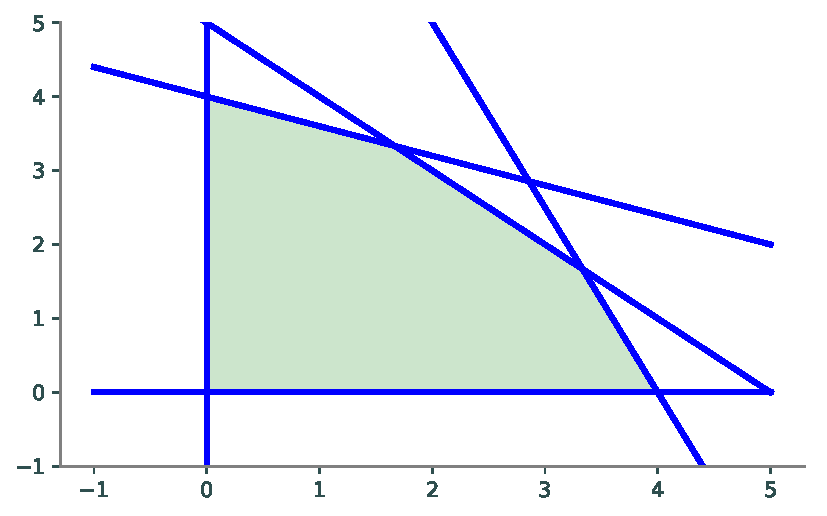
\includegraphics[width=\linewidth]{foundationsAppliedMathematicsLabs/Volume2/Simplex/figures/feasiblePolytope.pdf}
    \caption{The feasible region for a linear program with 2-dimensional constraints.}
\end{subfigure}%
\begin{subfigure}{.5\textwidth} % 3-d feasible polytope.
    \begin{center}
    \begin{tikzpicture}[dot/.style={circle,fill=blue,minimum size=3pt,inner sep=0pt, outer sep=-1pt}, >=stealth']

    \draw[blue!10!, fill=blue!5!](3,1)--(1.5,2.3)--(1.75,1.3)--cycle;
    \draw[blue!25!, fill = blue!15!](3,1)--(1.75,1.3)--(2.3,-1)--cycle;
    \draw[blue!55!, fill = blue!40!](1.75,1.3)--(2.3,-1)--(.8,-1)--cycle;
    \draw[blue!80!, fill = blue!65!](.8,-1)--(-.05,-.2)--(.25,.6)--(1.22,.06)--cycle;
    \draw[blue!85!, fill = blue!73!](-.05, -.2)--(-.3,0)--(.1, 1.65)--(.25, .6)--cycle;
    \draw[blue!65!, fill = blue!50!](.1,1.7)--(.25,.6)--(1.22,.07)--(1.75,1.3)--cycle;
    \draw[blue!40!, fill = blue!15!](.1,1.7)--(1.75,1.3)--(1.5,2.3)--cycle;

    \draw[-,thick](-.3,0)--(.1,1.7)--(1.5, 2.3)--(3, 1)--(2.3,-1)--(.8,-1)--cycle;

    \draw[-,thick](.1,1.7)--(3,1);
    \draw[-,thick](1.5, 2.3)--(2.3,-1);
    \draw[-,thick](.8,-1)--(1.74,1.3);
    \draw[-,thick](.1,1.7)--(.25,.6);
    \draw[-,thick](1.24,.07)--(.25,.6);
    \draw[-,thick](-.05,-.24)--(.25,.6);

    \draw[->](.37,.63)--(.22,1.61);
    \draw[->](.31,1.55)--(1.63,1.23);
    \draw[->](.75,-.85)--(1.12,.05);
    \draw[->](1.05,.05)--(.25,.48);
    \draw[->](1.83,1.35)--(1.65,2.1);

    \node[draw=none](x*)at(1.8,2.45){$\x^*$};

    \end{tikzpicture}
    \end{center}
    \caption{The feasible region for a linear program with 3-dimensional constraints.}
\end{subfigure}
\caption{If an optimal point exists, it is one of the vertices of the polyhedron.
The simplex algorithm searches for optimal points by moving between adjacent vertices in a direction that increases the value of the objective function until it finds an optimal vertex.}
\label{fig:polytope}
\end{figure}


To improve the solution, we:
\begin{enumerate}
    \item Select an entering variable with a negative reduced cost.
    \item Determine the leaving variable using the minimum ratio test.
    \item Perform a pivot operation to update the basis.
\end{enumerate}


This process continues until no negative reduced costs remain, indicating an optimal solution.


\subsection{Transforming the LP to Standard Form}

We start with the following linear program:
\begin{tcolorbox}[colback=orange!5!white, colframe=orange!75!black,    
    width=0.6\textwidth, % adjust width as desired
    box align=center, 
    title=\textbf{Linear Program to Solve}]

\[
\begin{aligned}
\text{Maximize}\quad & 2x + 3y \\
\text{subject to}\quad & x + y \;\;\;\;\;\;\;\;\;\;\; &&\leq 9, \\
& 2x + y \;\;\;\;\;\;\;\;\;\; &&\leq 16, \\
& x + 2y \;\;\;\;\;\;\;\;\; &&\leq 14, \\
& x, y \geq 0.
\end{aligned}
\]
\end{tcolorbox}
\begin{center}
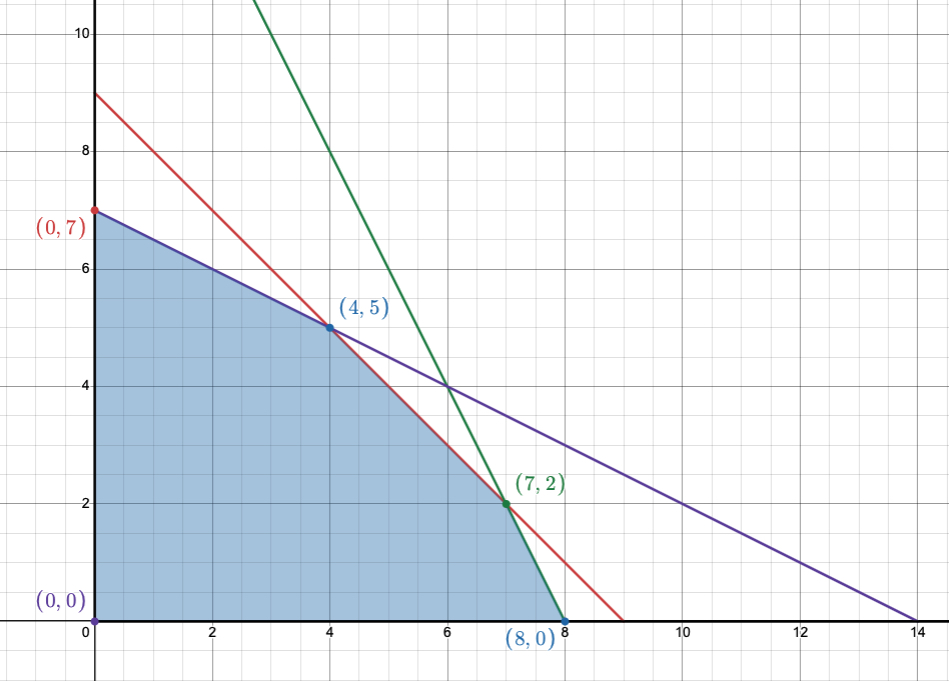
\includegraphics[scale = 0.3]{Figures/lp-feasible-desmos}
\end{center}
To convert these inequalities to equalities, we introduce slack variables \(s_1\), \(s_2\), and \(s_3\). Specifically, we rewrite each constraint as follows:

\[
\begin{aligned}
x + y + s_1 &= 9, \\
2x + y + s_2 &= 16, \\
x + 2y + s_3 &= 14,
\end{aligned}
\]
with the additional nonnegativity constraints \(s_1, s_2, s_3 \ge 0\). 

Hence, the linear program in standard form becomes:
\begin{tcolorbox}[
    colback=gray!5!white,
    colframe=gray!75!black,
    title=\textbf{Standard Form},
    width=0.6\textwidth, % adjust width as desired
    box align=center
]
\[
\begin{aligned}
\text{Maximize}\quad 
& 2x + 3y \\
\text{subject to}\quad 
& x + y + s_1 = 9, \\
& 2x + y + s_2 = 16, \\
& x + 2y + s_3 = 14, \\
& x, y, s_1, s_2, s_3 \ge 0.
\end{aligned}
\]
\end{tcolorbox}


\subsection*{Rewriting the System with \(\{s_1,s_2,s_3\}\) as the Basis}

When we say \(\{s_1,s_2,s_3\}\) is the basis, we solve each equation for the corresponding slack variable:
\[
\begin{aligned}
s_1 &= 9 \;-\; x \;-\; y, \\[6pt]
s_2 &= 16 \;-\; 2x \;-\; y,\\[6pt]
s_3 &= 14 \;-\; x \;-\; 2y.
\end{aligned}
\]
 Our initial non-basic variables are $x$ and $y$. 
We will call this representation of the linear program a \emph{dictionary}. 
\begin{tcolorbox}[colback=blue!5!white, colframe=blue!75!black,     width=0.6\textwidth, % adjust width as desired
    box align=center, title=\textbf{Initial Dictionary}]
\[
\begin{aligned}
\text{Maximize}\quad 
& z = 0 + 2x + 3y \\
\text{subject to}\quad 
& s_1 = 9 - x - y, \\
& s_2 = 16 - 2x - y, \\
& s_3 = 14 - x - 2y , \\
& x, y, s_1, s_2, s_3 \ge 0.
\end{aligned}
\]
From here we can read off a \emph{basic solution} that is 
$$
\text{Basic variables: } \ \ (s_1, s_2, s_3) = (9, 16,14),$$
$$
 \text{Non-basic variables:  } \ \ (x,y) = (0,0)
$$
with 
$$
\text{Objective value: } z = 0.
$$
Since the basic variables are all non-negative $(\geq 0)$, we call this a \emph{basic feasible solution}.
\end{tcolorbox}

\begin{remark}{Reading the Dictionary}{}
From the dictionary below, we can read off the corresponding \textbf{basic solution} and the \textbf{objective value}. The basic solution is obtained by:
\begin{itemize}
    \item Setting all \textbf{nonbasic variables} (those on the right-hand side of the equations, i.e., \(x\) and \(y\)) equal to zero.
    \item Reading off the values of the \textbf{basic variables} (\(s_1, s_2, s_3\)) from the right-hand side constants.
\end{itemize}

The dictionary is said to be \textbf{feasible} if all basic variables have nonnegative values (which is true here). Thus, this corresponds to a basic \emph{feasible} solution:
\[
x = 0, \quad y = 0, \quad s_1 = 9, \quad s_2 = 16, \quad s_3 = 14, \quad z = 0.
\]
\vspace{1cm}

\[
\begin{aligned}
\text{Maximize} \quad 
& \tikzmark{zstart} \text{\colorbox{green!20!white}{$z = 0$\phantom{$1_1$}}} ~ \text{\colorbox{gray!20!white}{$+ 2\tikzmark{x1}x + 3\tikzmark{y1}y \tikzmark{zend}$}} \\
\text{subject to} \quad 
& \tikzmark{s1start} \text{\colorbox{yellow}{$s_1 = 9$\phantom{1}}} ~ \tikzmark{s1rhs}\text{\colorbox{gray!20!white}{$- x - y$}} \tikzmark{s1end}, \\
& \tikzmark{s2start} \text{\colorbox{yellow}{$s_2 = 16$}} ~ \tikzmark{s2rhs} \text{\colorbox{gray!20!white}{$- 2x - y$}} \tikzmark{s2end}, \\
& \tikzmark{s3start} \text{\colorbox{yellow}{$s_3 = 14$}} ~ \tikzmark{s3rhs} \text{\colorbox{gray!20!white}{$- x - 2y$}} \tikzmark{s3end}, \\
& x, y, s_1, s_2, s_3 \ge 0.
\end{aligned}
\]

\begin{tikzpicture}[remember picture, overlay, >=stealth]

% Blue arrows: Basic variables and values
\draw[->, thick, blue] 
  ($(pic cs:s1rhs)+(-0.8,-0.1)$) -- ++(-3.5,-0.4) node[left, blue] {Basic var: $s_1 = 9$};
\draw[->, thick, blue] 
  ($(pic cs:s2rhs)+(-0.8,-0.10)$) -- ++(-3.5,-0.4) node[left, blue] {Basic var: $s_2 = 16$};
\draw[->, thick, blue] 
  ($(pic cs:s3rhs)+(-0.8,-0.10)$) -- ++(-3.5,-0.4) node[left, blue] {Basic var: $s_3 = 14$};

% Green arrow: Initial objective
\draw[->, thick, green!60!black] 
  ($(pic cs:zstart)+(0,0.1)$) -- ++(-2.5,1.0) node[left, green!50!black] {Initial objective: $z = 0$};

% Red arrows: Non-basic variables
\draw[->, thick, red] 
  ($(pic cs:x1)+(0,0.3)$) -- ++(1.2,1.2) node[right, red] {Non-basic: $x = 0$};
\draw[->, thick, red] 
  ($(pic cs:y1)+(0,0.3)$) -- ++(0.7,0.7) node[right, red] {Non-basic: $y = 0$};

\end{tikzpicture}
\end{remark}


 



%\subsection{Simplex Assuming Feasible Start}
%We now take as our \emph{initial} basic variables the three slack variables \(s_1, s_2, s_3\).  Geometrically, this corresponds to the point \(\,(x,y)=(0,0)\).  Indeed, if \(x=0\) and \(y=0\), then from the original constraints
%\[
%\begin{aligned}
%  x + y + s_1 &= 9,\\
%  2x + y + s_2 &= 16,\\
%  x + 2y + s_3 &= 14,  
%\end{aligned}
%\]
%it follows that
%\[
%s_1 = 9, 
%\quad
%s_2 = 16, 
%\quad
%s_3 = 14.
%\]
%All are nonnegative, so \(\,(s_1,s_2,s_3)\) is indeed a feasible basis, and \((0,0,9,16,14)\) is the \emph{basic feasible solution} (BFS).  
%
%\medskip
%
%
%Thus, in ``basic-variable \(=\) constant \(-\) (nonbasic terms)'' form, our system becomes
%
%\[
%\begin{cases}
%s_1 + x + y \;=\; 9,\\
%s_2 + 2x + y \;=\; 16,\\
%s_3 + x + 2y \;=\; 14.
%\end{cases}
%\]
%Since \(s_1, s_2, s_3\) are taken to be the \emph{basic} variables, the \emph{nonbasic} variables in this setup are \(x\) and \(y\).  Setting \(x=0,\,y=0\) immediately gives the BFS
%\[
%\bigl(x,y,s_1,s_2,s_3\bigr) 
%\;=\;
%(0,\,0,\,9,\,16,\,14).
%\]
%
%\subsection*{The Objective Function in this Basis}
%
%Our objective is:
%\[
%\text{Maximize}\quad z \;=\; 2x \;+\; 3y.
%\]
%Notice that in the current basis, the slack variables do not appear in the objective row (their cost coefficients are zero), so no extra terms involving \(s_1\), \(s_2\), or \(s_3\) appear in the \((z)\)-equation.  
%
%Hence, gathering all equations together in a simple ``dictionary-friendly'' format:
%
%\[
%\begin{aligned}
%&z = 0 \;+\; 2x \;+\; 3y,
%&s_1 \;+\; x \;+\; y \quad\;=\quad 9,\\
%&s_2 \;+\; 2x \;+\; y \quad=\quad 16,\\
%&s_3 \;+\; x \;+\; 2y \;=\; 14,\\
%\end{aligned}
%\]
%with the nonnegativity constraints
%\[
%x,\,y,\,s_1,\,s_2,\,s_3 \;\ge\;0.
%\]
%
%\paragraph{Value of \(\,z\) at the BFS \(\,(0,0,9,16,14)\).}
%At \(\,(x,y)=(0,0)\), we see \(z=2\cdot 0 + 3\cdot 0=0\).  So the initial objective value is
%\[
%z=0.
%\]
%From here, one would normally proceed with the \emph{simplex pivots} to drive the objective upwards (since this is a maximization problem).  We will handle those pivot steps next.
%
%\subsection*{Pivot Step: Letting \(y\) Enter and \(s_3\) Leave}
%
%We begin from the initial BFS where \(\{s_1,s_2,s_3\}\) are basic and \(\{x,y\}\) are nonbasic.  
%The system at that stage (with \(\,z = 2x + 3y\)) is:
%
%\[
%\begin{cases}
%s_1 = 9 \;-\; x \;-\; y,\\[4pt]
%s_2 = 16 \;-\; 2x \;-\; y,\\[4pt]
%s_3 = 14 \;-\; x \;-\; 2y,\\[4pt]
%z \;-\; 2x \;-\; 3y = 0.
%\end{cases}
%\]
At \(\bigl(x,y,s_1,s_2,s_3\bigr) = \bigl(0,0,9,16,14\bigr)\), the objective value is \(z=0\).

\subsection*{Choosing the Entering Variable}
\begin{tcolorbox}[colback=purple!5!white, colframe=purple!75!black, title=Entering Variable]

We examine the \emph{objective row} to determine which nonbasic variable should enter the basis. At this point, the objective is:
\[
z = 2x + 3y.
\]

\begin{itemize}
  \item The nonbasic variables are \(x\) and \(y\).
  \item Both have \textbf{positive} coefficients, which means that increasing either variable (while staying feasible) will increase the objective value \(z\).
  \item To decide between them, we apply a \textbf{pivot rule} — a strategy for selecting among eligible entering variables.
  
  \textbf{In this example, we use the \emph{Steepest Ascent} rule: we choose the nonbasic variable with the largest positive coefficient in the objective row.}
  
  \item Between \(x\) and \(y\), the coefficient of \(y\) is larger (\(3 > 2\)).
\end{itemize}

Therefore, we choose \(\boxed{y}\) to \textbf{enter} the basis.

\end{tcolorbox}

\subsubsection*{First Iteration. Ratio Test to Determine Who Leaves}

\begin{tcolorbox}[colback=yellow!5!white, colframe=yellow!75!black, title=\textbf{First Iteration - Ratio Test}]

We hold \(x = 0\) fixed and allow \(y\) to increase from \(0\).  
Then from the initial dictionary, the basic variables become (substituting \(x = 0\)):

\[
\begin{aligned}
s_1 &= 9 - y, \\
s_2 &= 16 - y, \\
s_3 &= 14 - 2y.
\end{aligned}
\]

To maintain feasibility, we require all basic variables to remain nonnegative:
\[
\begin{aligned}
s_1 \ge 0 &\;\implies\; 9 - y \ge 0 \;\implies\; y \le 9, \\
s_2 \ge 0 &\;\implies\; 16 - y \ge 0 \;\implies\; y \le 16, \\
s_3 \ge 0 &\;\implies\; 14 - 2y \ge 0 \;\implies\; y \le 14/2 = 7.
\end{aligned}
\]

The \emph{tightest constraint} is \(y \le 7\), which means \(s_3\) reaches zero first as \(y\) increases.  
Therefore, \(\boxed{s_3}\) will \textbf{leave the basis} in this pivot.

\end{tcolorbox}

This is called the \emph{Ratio Test} because we can compute these numbers as 
$$
9 - y = 0 \quad \Rightarrow y = 9 / 1 = 9
$$

$$
16 - y = 0 \quad \Rightarrow y = 16 / 1 = 16
$$

$$
14 - 2y = 0 \quad \Rightarrow y = 14 / 2 = 7
$$

If a coefficent on $y$ was positive, we would ignore that constraint as increasing $y$ would never violate the corresponding inequality.

The ratio test can also be thought of as changing the solution via a vector.  In particular, we are at the basic feasible solution $(s_1, s_2, s_3, x,y) = (9,16,14,0,0)$.  Now, as we increase $y$, we change the solution as 

$$
 (s_1, s_2, s_3, x,y) = (9,16,14,0,0) + \Delta y \cdot (-1, -1, -2, 0,1) = (9,16,14,0,0) + 7\cdot (-1, -1, -2, 0,1)  = (2,9,0,0,7).
$$
We will see these number appear as we pivot the dictionary to the new basis.

\subsection*{Pivoting on the \(s_3\)-Equation Solved for \(y\)}

Originally, \(s_3 + x + 2y = 14\).  Solve for \(y\):
\[
y \;=\; 7 \;-\; \tfrac{x}{2} \;-\; \tfrac{s_3}{2}.
\]
Substitute into the other rows (and the objective row), isolating each \emph{basic} variable on the left and all others on the right:
\[
\begin{aligned}
\text{Maximize}\quad 
& z = 0+ 2x + 3y \quad && = 21 + \frac{1}{2}x - \frac{3}{2}s_3 \\
\text{subject to}\quad 
& s_1 = 9 - x - y \quad && = 2 - \frac{1}{2}x + \frac{1}{2}s_3, \\
& s_2 = 16 - 2x - y \quad &&= 9 - \frac{3}{2}x + \frac{1}{2}s_3, \\
& s_3 = 14 - x - 2y \quad \Rightarrow y &&= 7 - \frac{1}{2}x - \frac{1}{2}s_3, \\
& x, y, s_1, s_2, s_3 \ge 0.
\end{aligned}
\]



\noindent
Hence the new \emph{basic variables} are \(\{z,\,y,\,s_1,\,s_2\}\) if we were to place \(z\) in the dictionary as well.  Typically, in a standard simplex dictionary, \(z\) is displayed in its own row, but it is not counted as a “basic variable” in the same sense as the constraints.  The nonbasic variables are now \(\{x,\,s_3\}\).

\subsection*{Updated Dictionary and Basic Feasible Solution}

\begin{tcolorbox}[colback=blue!5!white, colframe=blue!75!black, title=\textbf{Second Dictionary}]

\[
\begin{aligned}
\text{Maximize}\quad 
& z =  21 + \frac{1}{2}x - \frac{3}{2}s_3 \\
\text{subject to}\quad 
& s_1  = 2 - \frac{1}{2}x + \frac{1}{2}s_3, \\
& s_2  = 9 - \frac{3}{2}x + \frac{1}{2}s_3, \\
& y = 7 - \frac{1}{2}x - \frac{1}{2}s_3, \\
& x, y, s_1, s_2, s_3 \ge 0.
\end{aligned}
\]

\begin{itemize}
  \item Set \(\,x=0\) and \(\,s_3=0\) (the new nonbasic variables). 
  \item Then \(\,(y,s_1,s_2)\) become:
  \[
  y = 7, 
  \quad
  s_1 = 2,
  \quad
  s_2 = 9.
  \]
  \item Substitute in the objective row:
  \[
  z = 21 + \tfrac12\cdot 0 - \tfrac32\cdot 0 \;=\; 21.
  \]
\end{itemize}
Thus the new BFS after the pivot is 
\(\bigl(x,y,s_1,s_2,s_3\bigr) = \bigl(0,7,2,9,0\bigr)\) 
with \(z=21\).
\end{tcolorbox}

\subsection*{Second Iteration}
Since the objective function still has variables with positive coefficients in it, we will seek to pivot again to increase the objective.

\subsubsection*{Second Iteration. Identify the Entering Variable}
\begin{tcolorbox}[colback=purple!5!white, colframe=purple!75!black, title=\textbf{Second Iteration - Entering Variable}]
We look at the coefficients of the nonbasic variables in the \emph{objective} row,
\[
z = 21 \;+\; \tfrac12\,x \;-\;\tfrac32\,s_3.
\]
\begin{itemize}
  \item \(x\) has a \(\tfrac12\) coefficient (which is \textbf{positive}), 
  \item \(s_3\) has a \(-\tfrac32\) coefficient (negative).
\end{itemize}
Since this is a \emph{maximization} problem, increasing a variable with a \textbf{negative} objective coefficient would \emph{decrease} \(z\).  
Hence we choose \(x\), the only nonbasic variable with a positive coefficient, to \emph{enter} the basis.
\end{tcolorbox}
\subsubsection*{Second Iteration. Ratio Test to Determine Who Leaves}

\begin{tcolorbox}[colback=yellow!5!white, colframe=yellow!75!black, title=\textbf{Second Iteration - Ratio Test}]

We hold \(s_3=0\) for the moment and let \(x\) increase from \(0\).  
Then from the above system, the three basic variables become (substituting \(s_3=0\)):

\[
\begin{aligned}
y   &= 7 - \tfrac12\,x,\\
s_1 &= 2 - \tfrac12\,x,\\
s_2 &= 9 - \tfrac32\,x.
\end{aligned}
\]
We require these to remain nonnegative:
\[
\begin{aligned}
y \ge 0 \;&\implies\; 7 - \tfrac12\,x \;\ge\; 0 \;\implies\; x \;\le\; 7/\tfrac{1}{2} = 14,\\
s_1 \ge 0 \;&\implies\; 2 - \tfrac12\,x \;\ge\; 0 \;\implies\; x \;\le\; 2/\tfrac{1}{2} = 4,\\
s_2 \ge 0 \;&\implies\; 9 - \tfrac32\,x \;\ge\; 0 \;\implies\; x \;\le\; 9/\tfrac{3}{2} = 6.
\end{aligned}
\]
The \emph{smallest} upper bound is \(x \le 4\), which means \(\,s_1\) will reach zero first when \(x=4\).  
Hence \(\,s_1\) must \emph{leave} the basis.
\end{tcolorbox}
\subsubsection*{The Pivot: Solve the \(s_1\) Equation for \(x\)}

From
\[
s_1 = 2 \;-\;\tfrac12\,x \;+\;\tfrac12\,s_3,
\]
we isolate \(x\):
\[
s_1 - 2 - \tfrac12\,s_3 = -\,\tfrac12\,x
\quad\Longrightarrow\quad
x = -2\Bigl(s_1 - 2 - \tfrac12\,s_3\Bigr)
\;=\;
4 \;+\; s_3 \;-\; 2\,s_1.
\]
Rewriting,
\[
x \;+\; 2\,s_1 \;-\; s_3 
\;=\;
4.
\]
This \emph{becomes the new pivot row}, with \(x\) on the left side as a basic variable.

\subsubsection*{Eliminate \(x\) from the Other Rows}

Next, we substitute 
\(\;x = 4 + s_3 - 2\,s_1\;\)
into the rows for \(\{y,\,s_2,\,z\}\) to remove \(x\).  
(In each row, replace \(x\) by \(\,4 + s_3 - 2\,s_1\).)

\paragraph{Updating \(y\):}

Originally 
\[
y = 7 - \tfrac12\,x - \tfrac12\,s_3.
\]
Substitute \(x\):
\[
y
= 7 
- \tfrac12\bigl(4 + s_3 - 2s_1\bigr)
- \tfrac12\,s_3
=
7 - 2 - \tfrac12\,s_3 + s_1 - \tfrac12\,s_3
=
5 + s_1 - s_3.
\]
%Thus
%\[
%y 
%\;-\;
%s_1
%\;+\;
%s_3
%\;=\;
%5.
%\]

\paragraph{Updating \(s_2\):}

Originally
\[
s_2 = 9 - \tfrac32\,x + \tfrac12\,s_3.
\]
Substitute \(x\):
\[
s_2
= 9 
- \tfrac32\bigl(4 + s_3 - 2s_1\bigr)
+ \tfrac12\,s_3
= 
9 - 6 - \tfrac32\,s_3 + 3\,s_1 + \tfrac12\,s_3
=
3 + 3\,s_1 - s_3.
\]
%Hence
%\[
%s_2 
%\;-\;
%3\,s_1
%\;+\;
%s_3
%\;=\;
%3.
%\]

\paragraph{Updating the Objective Row \(\,z\):}

Originally
\[
z = 21 + \tfrac12\,x - \tfrac32\,s_3.
\]
Substitute \(x\):
\[
z
= 
21 
+ \tfrac12\bigl(4 + s_3 - 2s_1\bigr)
- \tfrac32\,s_3
=
21 + 2 + \tfrac12\,s_3 - s_1 - \tfrac32\,s_3
=
23 - s_1 - s_3.
\]
%Or
%\[
%z 
%\;+\;
%s_1
%\;+\;
%s_3
%\;=\;
%23.
%\]

\subsection*{The Third Dictionary}

\begin{tcolorbox}[colback=green!5!white, colframe=green!75!black, title=Final Dictionary]

After the pivot, the basic variables are now
\(\,\{\,x,\,y,\,s_2\}\), 
and the nonbasic variables are 
\(\,\{\,s_1,\,s_3\}\).  
Our updated equations, in a clean dictionary form (basic on the left) are:

\[
\begin{aligned}
\text{Maximize}\quad 
& z = 23 - s_1 - s_3 \\
\text{subject to}\quad 
& x = 4 - 2s_1 + s_3, \\
& y = 5 + s_1 - s_3, \\
& s_2 = 3 + 3s_1 - s_3, \\
& x, y, s_1, s_2, s_3 \geq 0.
\end{aligned}
\]

\begin{itemize}
  \item Setting the new nonbasic variables \(\,s_1=0\) and \(\,s_3=0\) gives
  \[
  x=4, \quad y=5,\quad s_2=3,\quad z=23.
  \]
  \item Thus our new BFS is 
  \(\bigl(x,y,s_1,s_2,s_3\bigr)=\bigl(4,\,5,\,0,\,3,\,0\bigr)\) 
  with objective value \(z=23\).
\end{itemize}
\end{tcolorbox}

\begin{remark}{Reading the Final Dictionary}{}
From the final dictionary below, we read the solution using the same process:
\begin{itemize}
    \item Set all \textbf{nonbasic variables} equal to zero. Here, the nonbasic variables are \(s_1\) and \(s_3\).
    \item Evaluate the values of the basic variables \(x, y, s_2\) and the objective \(z\).
\end{itemize}

This yields the final basic feasible solution:
\[
s_1 = 0, \quad s_3 = 0, \quad x = 4, \quad y = 5, \quad s_2 = 3, \quad z = 23.
\]

\vspace{1cm}

\[
\begin{aligned}
\text{Maximize} \quad 
& \tikzmark{zstart2} \text{\colorbox{green!20!white}{$z = 23$}} ~ \text{\colorbox{gray!20!white}{$- s_1 - s_3$}} \tikzmark{zend2} \\
\text{subject to} \quad 
& \tikzmark{x2} \text{\colorbox{yellow}{$x = 4$}} ~ \text{\colorbox{gray!20!white}{$- 2s_1 + s_3$}}, \\
& \tikzmark{y2} \text{\colorbox{yellow}{$y = 5$}} ~ \text{\colorbox{gray!20!white}{$+ s_1 - s_3$}}, \\
& \tikzmark{s22} \text{\colorbox{yellow}{$s_2 = 3$}} ~ \text{\colorbox{gray!20!white}{$+ 3s_1 - s_3$}}, \\
& x, y, s_1, s_2, s_3 \ge 0.
\end{aligned}
\]

\begin{tikzpicture}[remember picture, overlay, >=stealth]

% Green arrow: Final objective
\draw[->, thick, green!60!black] 
  ($(pic cs:zstart2)+(0,0.1)$) -- ++(-2.5,1.0) node[left, green!50!black] {Final objective: $z = 23$};

% Yellow arrows: Basic variables
\draw[->, thick, blue] 
  ($(pic cs:x2)+(-0.2,-0.2)$) -- ++(-3.0,-0.5) node[left, blue] {Basic var: $x = 4$};
\draw[->, thick, blue] 
  ($(pic cs:y2)+(-0.2,-0.2)$) -- ++(-3.0,-0.5) node[left, blue] {Basic var: $y = 5$};
\draw[->, thick, blue] 
  ($(pic cs:s22)+(-0.2,-0.2)$) -- ++(-3.0,-0.5) node[left, blue] {Basic var: $s_2 = 3$};

% Red arrows: Non-basic variables
\draw[->, thick, red] 
  ($(pic cs:zend2)+(0.2,0.3)$) -- ++(1.2,1.0) node[right, red] {Non-basic: $s_1 = 0$};
\draw[->, thick, red] 
  ($(pic cs:zend2)+(0.4,0.1)$) -- ++(1.5,0.5) node[right, red] {Non-basic: $s_3 = 0$};

\end{tikzpicture}

\vspace{1em}

\textbf{Why is this optimal?}  
This is a maximization problem, and the final dictionary expresses the objective as:
\[
z = 23 - s_1 - s_3.
\]
Both \(s_1\) and \(s_3\) are nonbasic and currently zero. Since increasing either would \emph{decrease} the value of \(z\), we cannot improve the objective by pivoting.  
\\[0.5em]
\textbf{Hence, this solution is optimal.}
\end{remark}


\subsection{Summarizing the steps taken}
We now summarize the whole process:

\begin{enumerate}
    \item \textbf{Original LP}  
    \begin{tcolorbox}[colback=orange!5!white, colframe=orange!75!black,    
    width=0.6\textwidth, % adjust width as desired
    box align=center, 
    title=\textbf{Linear Program to Solve}]
    \[
    \begin{aligned}
    \text{Maximize} \quad & 2x + 3y \\
    \text{subject to} \quad 
    & x + y \leq 9, \\
    & 2x + y \leq 16, \\
    & x + 2y \leq 14, \\
    & x, y \geq 0.
    \end{aligned}
    \]
    \end{tcolorbox}

    \item \textbf{Standard Form with Feasible Basis $\{s_1, s_2, s_3\}$}  
    \begin{tcolorbox}[colback=gray!5!white, colframe=gray!75!black,    
    width=0.6\textwidth, % adjust width as desired
    box align=center, 
    title=\textbf{Standard Form}]
    \[
    \begin{aligned}
    \text{Maximize} \quad & 2x + 3y \\
    \text{subject to} \quad 
    & x + y + s_1 = 9, \\
    & 2x + y + s_2 = 16, \\
    & x + 2y + s_3 = 14, \\
    & x, y, s_1, s_2, s_3 \geq 0.
    \end{aligned}
    \]
    \end{tcolorbox}

    \item \textbf{Initial Dictionary with Basis \( (s_1, s_2, s_3) \)}
    \begin{tcolorbox}[colback=blue!5!white, colframe=blue!75!black,    
    width=0.6\textwidth, % adjust width as desired
    box align=center, 
    title=\textbf{Initial Dictionary}]
    \[
    \begin{aligned}
    \text{Maximize} \quad & z = 0 + 2x + 3y \\
    \text{subject to} \quad 
    & s_1 = 9 - x - y, \\
    & s_2 = 16 - 2x - y, \\
    & s_3 = 14 - x - 2y.\\
    & x,y,s_1, s_2, s_3 \geq 0
    \end{aligned}
    \]
    \end{tcolorbox}
    Basic Feasible Solution: \( (s_1, s_2, s_3) = (9,16,14), (x,y) = (0,0) \)  
    Objective Value: \( z = 0 \).\\  
    Since the objective row has a positive coefficient, it is not optimal.
    
    \item \textbf{First Iteration:}
\begin{enumerate}
    \item \textbf{Ratio Test:} \( y \) enters, \( s_3 \) leaves.

    \item \textbf{Dictionary after Pivoting \( y \) in, \( s_3 \) out}  
    \begin{tcolorbox}[colback=blue!5!white, colframe=blue!75!black,    
    width=0.6\textwidth, % adjust width as desired
    box align=center, 
    title=\textbf{Second Dictionary}]
    \[
    \begin{aligned}
    \text{Maximize} \quad & z = 21 + \frac{1}{2}x - \frac{3}{2}s_3 \\
    \text{subject to} \quad 
    & s_1 = 2 - \frac{1}{2}x + \frac{1}{2}s_3, \\
    & s_2 = 9 - \frac{3}{2}x + \frac{1}{2}s_3, \\
    & y = 7 - \frac{1}{2}x - \frac{1}{2}s_3.
    \end{aligned}
    \]
    \end{tcolorbox}
    Basic Feasible Solution: \( (s_1, s_2, y) = (2,9,7), (x,s_3) = (0,0) \)  
    Objective Value: \( z = 21 \).\\ 
    Since the objective row has a positive coefficient, it is not optimal.  
    \end{enumerate}
    \item \textbf{Second Iteration}
    \begin{enumerate}
    \item \textbf{Ratio Test:} \( x \) enters, \( s_1 \) leaves.

    \item \textbf{Final Dictionary (Optimal) after pivoting $x$ in, $s_1$ out.} 
    \begin{tcolorbox}[colback=green!5!white, colframe=green!75!black,    
    width=0.6\textwidth, % adjust width as desired
    box align=center, 
    title=\textbf{Final Dictionary}] 
    \[
    \begin{aligned}
    \text{Maximize} \quad & z = 23 + s_1 + s_3 \\
    \text{subject to} \quad 
    & x = 4 - 2s_1 + s_3, \\
    & y = 5 + s_1 - s_3, \\
    & s_2 = 3 + 3s_1 - s_3.
    \end{aligned}
    \]
    \end{tcolorbox}
    Basic Feasible Solution: \( (x,y,s_2) = (4,5,3), (s_1,s_3) = (0,0) \)  
    Objective Value: \( z = 23 \).\\ 
    Since all coefficients in the objective row are non-positive, this is the optimal solution.
    \end{enumerate}
\end{enumerate}

\begin{resource}
You  can review these calculations using the code avaibale here in Jupyter Notebook Format.
\begin{itemize}
\item \href{https://colab.research.google.com/drive/1kUWeNOVZByIoSWWUEUEFwwdFhAQvGcsG?usp=sharing}{Colab Version (online)}
\item \href{https://github.com/open-optimization/open-optimization-or-examples/blob/master/linear-programming/Simplex_Tableaus_From_Basis.ipynb}{Jupyter Notebook for Download}
\end{itemize}
\end{resource}


\section{ The Simplex Algorithm!}
Here we formally describe the simplex algorithm.
\begin{algorithm}[H]
\caption{Simplex Algorithm}
\begin{algorithmic}[1]
\State \textbf{Input:} Linear program in standard form with a feasible starting basis (typically the slack variables).
\State \textbf{Initialization:} Reformulate the system in dictionary form:
  \begin{itemize}
    \item Write the equations with the basic variables on the left and the nonbasic variables on the right.
    \item Substitute the basic variables into the objective function.
  \end{itemize}
\Repeat
  \State \textbf{1. Choose the entering variable:} Select a nonbasic variable with a positive coefficient in the objective row.
  \State \textbf{2. Determine the leaving variable:} For each basic variable, perform the ratio test by calculating
  \[
  \text{ratio} = \frac{\text{current value of basic variable}}{\text{coefficient of entering variable (if positive)}}
  \]
  The basic variable that reaches zero first (i.e., the smallest ratio) is chosen to leave the basis.
  \State \textbf{3. Pivot:} 
  \begin{itemize}
    \item Rewrite the equation of the leaving variable so that it is expressed in terms of the entering variable.
    \item Substitute this expression into all other equations and the objective function.
  \end{itemize}
\Until{All coefficients in the objective row for nonbasic variables are non-positive (indicating that an optimal solution has been reached).}
\State \textbf{Output:} The optimal solution.
\end{algorithmic}
\end{algorithm}


We dive a little deeper into what the ratio test is here:
\begin{itemize}
    \item \textbf{The Ratio Test (Formal Definition)}  

    The Ratio Test is used to determine which basic variable should leave the basis when a nonbasic variable enters. It ensures that we maintain feasibility by preventing any basic variables from becoming negative.

    Given a \emph{pivot column} corresponding to the entering variable (say, \( x_e \)), the Ratio Test is defined as follows:

    \begin{itemize}
        \item Identify all constraints of the form:
        \[
        s_i = b_i - a_{i,e} x_e
        \]
        where \( b_i \) is the right-hand side value, and \( a_{i,e} \) is the coefficient of the entering variable in row \( i \).
        \item Compute the ratio for all constraints where \( a_{i,e} > 0 \):
        \[
        \frac{b_i}{a_{i,e}}
        \]
        \item The \emph{leaving variable} corresponds to the row that gives the \emph{smallest positive ratio}. This ensures that the increase in \( x_e \) does not cause any basic variable to become negative.
    \end{itemize}

    \textbf{Special Cases:}
    \begin{itemize}
        \item If all \( a_{i,e} \leq 0 \), then the problem is \emph{unbounded}, meaning the objective function can be increased indefinitely.
        \item If multiple rows attain the same minimum ratio, a \emph{tie-breaking rule} is needed (e.g., Bland’s Rule to avoid cycling).
    \end{itemize}

    The Ratio Test guarantees that we always select the proper constraint to maintain feasibility while pivoting towards an improved solution.
\end{itemize}

\begin{learningcheckpoint}{Ratio Test and Infeasible Solutions}
When applying the simplex method, why might choosing the wrong leaving variable during the ratio test lead you to an \emph{infeasible} basic solution?  

\emph{Hint: Think about what the ratio test is meant to guarantee for the nonnegativity of variables after the pivot.}
\end{learningcheckpoint}



We will see another example of this, and then modify it to handle LPs that don't have a simple initial basic feasible solution.

%\section*{Simplex Algorithm Execution}
%
%\subsection*{Initial Problem}
%\[
%\begin{aligned}
%\text{Maximize}\quad & 2x + 3y \\
%\text{subject to}\quad & s_1 = 9 - x - y, \\
%                        & s_2 = 16 - 2x - y, \\
%                        & s_3 = 14 - x - 2y, \\
%                        & x, y, s_1, s_2, s_3 \ge 0.
%\end{aligned}
%\]
%
%\noindent We start with a feasible basis (the slack variables).
%
%\subsection*{Iteration 1: Entering \(y\) and Leaving \(s_3\)}
%Choose \(y\) to increase.
%
%Based on the ratio test, choose \(s_3\) to leave the basis and let \(y\) enter the basis.
%
%Rewrite the equation for \(s_3\):
%\[
%s_3 = 14 - x - 2y
%\]
%becomes
%\[
%y = 7 - 0.50x - 0.50s_3.
%\]
%
%Now substitute this expression into the rest of the dictionary to obtain
%\[
%\begin{aligned}
%\text{Maximize}\quad & 21 + 0.50x - 1.50s_3 \\
%\text{subject to}\quad & s_1 = 2 - 0.50x + 0.50s_3, \\
%                        & s_2 = 9 - 1.50x + 0.50s_3, \\
%                        & y = 7 - 0.50x - 0.50s_3, \\
%                        & x, y, s_1, s_2, s_3 \ge 0.
%\end{aligned}
%\]
%
%\subsection*{Iteration 2: Entering \(x\) and Leaving \(s_1\)}
%Next, pick \(x\) to increase. This means that \(x\) enters the basis and \(s_1\) leaves the basis.
%
%The new dictionary is
%\[
%\begin{aligned}
%\text{Maximize}\quad & 23 - s_1 - s_3 \\
%\text{subject to}\quad & x = 4 - 2s_1 + s_3, \\
%                        & s_2 = 3 + 3s_1 - s_3, \\
%                        & y = 5 + s_1 - s_3, \\
%                        & x, y, s_1, s_2, s_3 \ge 0.
%\end{aligned}
%\]
%
%\noindent This is optimal!
%
%


In the example worked out in the prior section, we used the \emph{steepest ascent} pivot rule, which means that we always used the variable in the objective with the largest postive coefficient to enter the basis.  However, we could make other choices instead.  The choice of how to pivot is left a little ambigious in the simplex method and many different pivot rules have been proposed.
See Exercise~\ref{ex:alternative-pivot} to see how the simplex method plays out when pivoting in a different direction first.  

In fact, in the figure below, we show the simplex dictionary at every single vertex.  You can see that from any vertex, you can pivot along an edge of the feasible region to another vertex.
\begin{center}
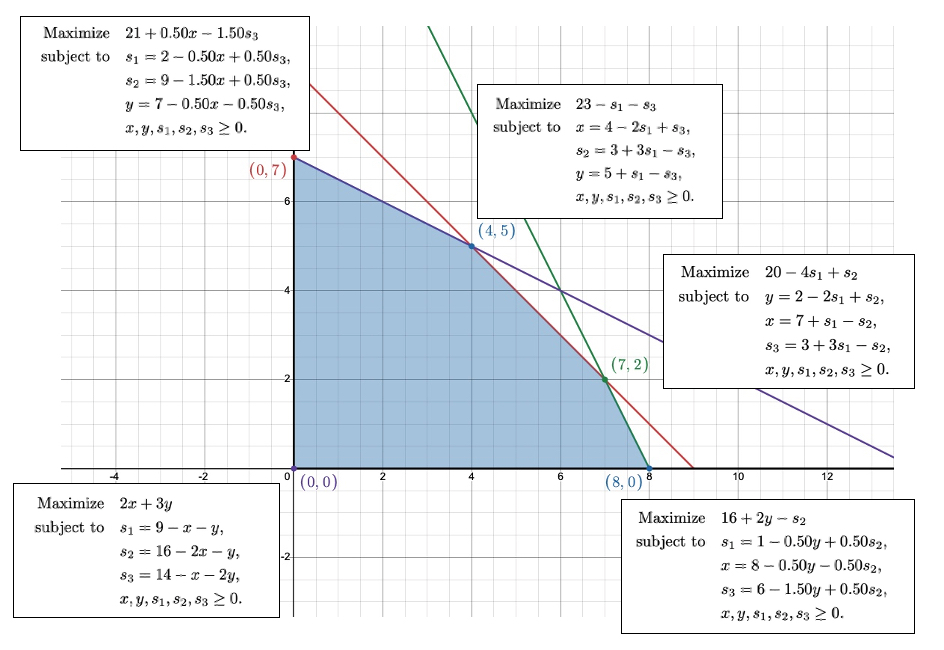
\includegraphics[scale = 0.5]{Figures/simplex-all-tableaus}
\end{center}

\begin{remark}{Reduced Costs}{def:reduced-cost}
The coefficients of the nonbasic variables in the objective row are their \emph{reduced costs}:
\[
\text{Reduced cost of } s_1 = -1, \quad \text{Reduced cost of } s_3 = -1.
\]

\[
\begin{aligned}
\text{Maximize} \quad 
& z = 23~ \text{\colorbox{purple!20!white}{$- s_1 - s_3$}} \tikzmark{zend2} \\
\text{subject to} \quad 
& \tikzmark{x2} x = 4 ~ - 2s_1 + s_3, \\
& \tikzmark{y2} y = 5 ~ + s_1 - s_3, \\
& \tikzmark{s22} s_2 = 3~ + 3s_1 - s_3, \\
& x, y, s_1, s_2, s_3 \ge 0.
\end{aligned}
\]

%\begin{tikzpicture}[remember picture, overlay, >=stealth]
%% Red arrows: Non-basic variables
%\draw[->, thick, red] 
%  ($(pic cs:zend2)+(0.2,0.3)$) -- ++(1.2,0.1) node[right, red] {Non-basic: $s_1 = 0$};
%\draw[->, thick, red] 
%  ($(pic cs:zend2)+(0.4,0.1)$) -- ++(1.5,-0.5) node[right, red] {Non-basic: $s_3 = 0$};
%
%\end{tikzpicture}

\bigskip


\begin{itemize}
    \item These values indicate how much the objective \( z \) would change per unit increase in the corresponding variable, assuming all others are held fixed and feasibility is maintained.
    \item Because this is a maximization problem, a \emph{negative} reduced cost implies that increasing the variable would \emph{decrease} the objective.
\end{itemize}

\medskip

\noindent\textbf{Optimality Condition:}  
A basic feasible solution is optimal if and only if all reduced costs of nonbasic variables satisfy:
\[
\text{(for maximization):} \quad \text{reduced cost} \le 0.
\]

\medskip

In this dictionary:
\[
\text{Reduced costs of } s_1, s_3 < 0 \quad \Rightarrow \quad \text{no nonbasic variable can enter to improve } z.
\]

\textbf{Therefore, the current solution is optimal.}
\end{remark}

\begin{definition}{Reduced Costs in an Arbitrary Dictionary}{def:reduced-cost-general}

Let a linear program in standard form be given by
\[
\text{Maximize} \quad \mathbf{c}^\top \mathbf{x} \quad \text{subject to} \quad A\mathbf{x} = \mathbf{b}, \quad \mathbf{x} \geq 0,
\]
and let \( B \subseteq \{1, \dots, n\} \) be a basis of linearly independent columns of \( A \). The corresponding \emph{dictionary} expresses the basic and objective variables in terms of the nonbasic variables \( N = \{1, \dots, n\} \setminus B \):

\[
\begin{aligned}
z &= z_0 + \sum_{j \in N} \bar{c}_j x_j \\
x_i &= \bar{b}_i + \sum_{j \in N} \bar{a}_{ij} x_j \quad \text{for } i \in B
\end{aligned}
\]

Here:
\begin{itemize}
    \item \( x_i \) are the basic variables,
    \item \( x_j \) for \( j \in N \) are the nonbasic variables,
    \item \( z_0 \) is the current value of the objective,
    \item \( \bar{c}_j \) is the \emph{reduced cost} of variable \( x_j \), and
    \item \( \bar{b}_i \) is the value of basic variable \( x_i \) when \( x_j = 0 \) for all \( j \in N \).
\end{itemize}
\end{definition}




\section{No Feasible Initial Basis and the Big-M Method}
\begin{outcome}
\begin{itemize}
\item Address case where initial basis is infeasible
\item Modify the simplex algorithm using the Big-M method to find a feasible starting basis
\begin{itemize}
\item Introduce artificial varibales to rows that violate initial feasibility
\item Add large penalty (Big-M) to the objective on these artificial variables
\item Run Simplex and pivot until can remove artificial variables
\item Drop the auxillary variables and proceed with the simplex algorithm
\end{itemize}
\end{itemize}
\end{outcome}
Consider the linear program
\begin{tcolorbox}[colback=orange!5!white, colframe=orange!75!black,    
    width=0.6\textwidth, % adjust width as desired
    box align=center, 
    title=\textbf{Original Linear Program}]
\[
\begin{aligned}
\text{Maximize}\quad & 2x + 3y \\
\text{subject to}\quad & 2x + y \;\;\;\;\;\;\;\;\;\;\; \geq 5, \\
& 2x + y \;\;\;\;\;\;\;\;\;\; \leq 16, \\
& x + 2y \;\;\;\;\;\;\;\;\; \leq 14, \\
& x, y \geq 0.
\end{aligned}
\]
\end{tcolorbox}

\begin{center}
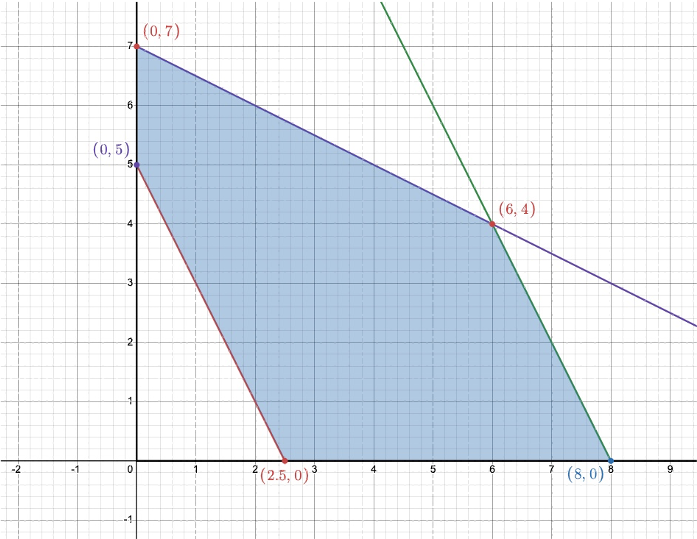
\includegraphics[scale = 1]{Figures/big-M}
\end{center}
Unfortunately, the origin is not feasible!!!


We rewrite the first inequality as
\[
-2x - y \leq -5,
\]
so that all constraints are of the form “$\le$”. Then, introducing slack variables, we have
\begin{tcolorbox}[colback=red!5!white, colframe=red!75!black,    
    width=0.6\textwidth, % adjust width as desired
    box align=center, 
    title=\textbf{Infeasible Dictionary!}]
\[
\begin{aligned}
\text{Maximize}\quad & 2x + 3y \\
\text{subject to}\quad & s_1 = -5 + 2x + y,\\[1mm]
& s_2 = 16 - 2x - y,\\[1mm]
& s_3 = 14 - x - 2y,\\[1mm]
& x,\, y,\, s_1,\, s_2,\, s_3 \geq 0.
\end{aligned}
\]
\end{tcolorbox}
\textbf{At the starting point \(x = y = 0\), we have \(s_1 = -5\), so the basic solution is infeasible!}

\subsection*{Introducing an Artificial Variable}

To obtain a feasible initial basis, we add an artificial variable \(a_1 \ge 0\) to the first constraint:
\[
s_1 = -5 + 2x + y + a_1.
\]
This new variable can be though of as altering the right hand side of the inequality as much as needed by "cheating" and making the initial basis feasible.

Simultaneously, we modify the objective function by adding a large penalty \(-1000a_1\) (here, \(M=1000\)) so that the optimal solution forces \(a_1\) to zero:
\begin{tcolorbox}[colback=pink!5!white, colframe=pink!75!black,    
    width=0.6\textwidth, % adjust width as desired
    box align=center, 
    title=\textbf{Artificial Dictionary - Need to Pivot $a_1$ into basis}]
\[
\begin{aligned}
\text{Maximize}\quad & 2x + 3y - 1000a_1 \\
\text{subject to}\quad & s_1 = -5 + 2x + y + a_1,\\[1mm]
& s_2 = 16 - 2x - y,\\[1mm]
& s_3 = 14 - x - 2y,\\[1mm]
& x,\, y,\, s_1,\, s_2,\, s_3,\, a_1 \ge 0.
\end{aligned}
\]
\end{tcolorbox}

\subsection*{Changing the Basis}

Next, we change the basis to one that is feasible. After some pivoting, we may arrive at a dictionary like:
\begin{tcolorbox}[colback=blue!5!white, colframe=pink!75!black,    
    width=0.6\textwidth, % adjust width as desired
    box align=center, 
    title=\textbf{Initial Artificial Dictionary}]
\[
\begin{aligned}
\text{Maximize}\quad & -5000 + 2002x + 1003y - 1000s_1 \\
\text{subject to}\quad & a_1 = 5 - 2x - y + s_1,\\[1mm]
& s_2 = 16 - 2x - y,\\[1mm]
& s_3 = 14 - x - 2y,\\[1mm]
& x,\, y,\, s_1,\, s_2,\, s_3,\, a_1 \ge 0.
\end{aligned}
\]
\end{tcolorbox}
With further pivoting, we obtain a dictionary where \(a_1\) is nonbasic:
\begin{tcolorbox}[colback=blue!5!white, colframe=pink!75!black,    
    width=0.6\textwidth, % adjust width as desired
    box align=center, 
    title=\textbf{Second Artificial Dictionary}]
\[
\begin{aligned}
\text{Maximize}\quad & 5 + 2y + s_1 - 1001a_1 \\
\text{subject to}\quad & x = 2.50 - 0.50y + 0.50s_1 - 0.50a_1,\\[1mm]
& s_2 = 11 - s_1 + a_1,\\[1mm]
& s_3 = 11.50 - 1.50y - 0.50s_1 + 0.50a_1,\\[1mm]
& x,\, y,\, s_1,\, s_2,\, s_3,\, a_1 \ge 0.
\end{aligned}
\]
\end{tcolorbox}
Since \(a_1\) is now nonbasic (and hence \(a_1=0\) in the basic solution), the basis is feasible.

\begin{remark}{Artificial Variable Can Be Removed — Feasible Start for Phase II}{}
This is the second artificial dictionary from \textbf{Phase I} of the two-phase simplex method. Our goal was to eliminate the artificial variable \(a_1\) while finding a feasible solution to the original problem.

Let’s analyze this dictionary:
\begin{itemize}
    \item The artificial variable \(a_1\) appears in the system, but it is \textbf{not basic}.
    \item Because \(a_1\) is a nonbasic variable and its value is currently zero, it can be \textbf{removed} from the dictionary without violating feasibility.
    \item All basic variables (\(x, s_2, s_3\)) have nonnegative values when \(a_1 = 0\), and all coefficients of \(a_1\) can simply be deleted.
\end{itemize}

\textbf{Conclusion:} We now have a basic feasible solution to the original problem (with no artificial variables present), so we can begin \textbf{Phase II of the simplex method} using this dictionary as the starting point.

\vspace{1cm}

\[
\begin{aligned}
\text{Maximize} \quad 
& \tikzmark{zstart4} \text{\colorbox{green!20!white}{$5$}} ~ \text{\colorbox{gray!20!white}{$+ 2y + s_1 - 1001a_1$}} \tikzmark{zend4} \\
\text{subject to} \quad 
& \tikzmark{xx4} \text{\colorbox{yellow}{$x = 2.50$}} ~ \text{\colorbox{gray!20!white}{$- 0.50y + 0.50s_1 - 0.50a_1$}},\\[1mm]
& \tikzmark{s24} \text{\colorbox{yellow}{$s_2 = 11$}} ~ \text{\colorbox{gray!20!white}{$- s_1 + a_1$}},\\[1mm]
& \tikzmark{s34} \text{\colorbox{yellow}{$s_3 = 11.50$}} ~ \text{\colorbox{gray!20!white}{$- 1.50y - 0.50s_1 + 0.50a_1$}},\\[1mm]
& x,\, y,\, s_1,\, s_2,\, s_3,\, a_1 \ge 0.
\end{aligned}
\]

\begin{tikzpicture}[remember picture, overlay, >=stealth]

% Arrows: basic variables
\draw[->, thick, blue] 
  ($(pic cs:xx4)+(-0.2,-0.2)$) -- ++(-3.0,-0.5) node[left, blue] {Basic var: $x = 2.50$};
\draw[->, thick, blue] 
  ($(pic cs:s24)+(-0.2,-0.2)$) -- ++(-3.0,-0.5) node[left, blue] {Basic var: $s_2 = 11$};
\draw[->, thick, blue] 
  ($(pic cs:s34)+(-0.2,-0.2)$) -- ++(-3.0,-0.5) node[left, blue] {Basic var: $s_3 = 11.50$};

% Red arrow: nonbasic artificial variable
\draw[->, thick, red] 
  ($(pic cs:zend4)+(0.4,0.3)$) -- ++(2,0.5) node[right, red] {Non-basic: $a_1 = 0$};

\end{tikzpicture}
\end{remark}

\begin{learningcheckpoint}
Why can the artificial variable be removed from this system?
\end{learningcheckpoint}

\subsection*{Removing the Artificial Variable}

Once feasibility is achieved, we remove the artificial variable from the formulation. This yields:
\begin{tcolorbox}[colback=blue!5!white, colframe=blue!75!black,    
    width=0.6\textwidth, % adjust width as desired
    box align=center, 
    title=\textbf{First Feasible Dictionary!}]
\[
\begin{aligned}
\text{Maximize}\quad & 5 + 2y + s_1 \\
\text{subject to}\quad & x = 2.50 - 0.50y + 0.50s_1,\\[1mm]
& s_2 = 11 - s_1,\\[1mm]
& s_3 = 11.50 - 1.50y - 0.50s_1,\\[1mm]
& x,\, y,\, s_1,\, s_2,\, s_3 \ge 0.
\end{aligned}
\]
\end{tcolorbox}
Now, with a feasible starting basis in hand, the standard simplex method can be applied to find the optimal solution.

\begin{tcolorbox}[colback=purple!5!white, colframe=purple!75!black,    
    width=0.6\textwidth, % adjust width as desired
    box align=center, 
    title=\textbf{First Feasible Iteration - Choose entering variable}]

We choose $y$ to enter the basis since it has the largest positive coefficient in the objective of $2$.
\end{tcolorbox}
\begin{exercise}{Complete the simplex method}{}
Complete the simplex method for this problem by carrying out 3 more pivots using the steepest ascent pivot rule.
\end{exercise}

\newpage

\section*{Big-M Method Algorithm}

\begin{algorithm}[H]
\caption{Big-M Method for Linear Programming}
\begin{algorithmic}[1]
\State \textbf{Input:} Linear program in standard form (maximize), possibly with an infeasible initial basic solution.
\State \textbf{Preprocessing:}
    \begin{itemize}
        \item For each constraint that yields a negative right-hand side, multiply the constraint by \(-1\) so that the right-hand side becomes positive.
        \item For each constraint without an obvious feasible basic variable, add an artificial variable \(a_i \ge 0\).
    \end{itemize}
\State \textbf{Modify the Objective Function:}
    \begin{itemize}
        \item Add a penalty term \(-M a_i\) (with \(M\) a very large constant) for each artificial variable to the original objective.
    \end{itemize}
\State \textbf{Formulate the Initial Dictionary:}
    \begin{itemize}
        \item Include slack (or surplus) variables and artificial variables.
        \item Use the modified objective function.
    \end{itemize}
\State \textbf{Compute an Initial Basis:}
    \begin{itemize}
        \item Choose basic variables so that the artificial variables are initially in the basis if necessary.
    \end{itemize}
\While{an artificial variable is in the basis or the current basic solution is infeasible}
    \State Perform a simplex pivot that moves at least one artificial variable out of the basis
    \Comment{Pivot as in the standard simplex method but using the modified objective function.}
\EndWhile
\State \textbf{Remove Artificial Variables:}
    \begin{itemize}
        \item Once a feasible basis is obtained (i.e., all artificial variables are zero), remove the columns corresponding to the artificial variables.
    \end{itemize}
\State \textbf{Proceed with the Standard Simplex Method:}
    \begin{itemize}
        \item Continue simplex iterations using the original objective function (without the artificial variables).
    \end{itemize}
\State \textbf{Output:} The optimal solution for the original problem, or a declaration that the problem is infeasible if any artificial variable remains positive.
\end{algorithmic}
\end{algorithm}

%
%\section{No feasible initial basis}
%
%
%\[
%\begin{aligned}
%\text{Maximize}\quad & 2x + 3y \\
%\text{subject to}\quad & 2x + y \;\;\;\;\;\;\;\;\;\;\; \geq 5, \\
%& 2x + y \;\;\;\;\;\;\;\;\;\; \leq 16, \\
%& x + 2y \;\;\;\;\;\;\;\;\; \leq 14, \\
%& x, y \geq 0.
%\end{aligned}
%\]
%
%
%\[
%\begin{aligned}
%\text{Maximize}\quad & 2x + 3y \\
%\text{subject to}\quad & -2x - y \;\;\;\;\;\;\;\;\;\;\; \leq -5, \\
%& 2x + y \;\;\;\;\;\;\;\;\;\; \leq 16, \\
%& x + 2y \;\;\;\;\;\;\;\;\; \leq 14, \\
%& x, y \geq 0.
%\end{aligned}
%\]
%
%
%
%\[
%\begin{aligned}
%\text{Maximize}\quad & + 2x + 3y \\
%\text{subject to}\quad & s_1 = -5 + 2x + y,\\ 
%& s_2 = 16 - 2x - y,\\ 
%& s_3 = 14 - x - 2y,\\ 
%& x, y, s_1, s_2, s_3 \ge 0.
%\end{aligned}
%\]
%
%Add an artificial variable!
%
%\[
%\begin{aligned}
%\text{Maximize}\quad & + 2x + 3y - 1000a_1 \\
%\text{subject to}\quad & s_1 = -5 + 2x + y + a_1,\\ 
%& s_2 = 16 - 2x - y,\\ 
%& s_3 = 14 - x - 2y,\\ 
%& x, y, s_1, s_2, s_3, a_1 \ge 0.
%\end{aligned}
%\]
%Now we can change the basis to something feasible (without thinking too hard).
%
%\[
%\begin{aligned}
%\text{Maximize}\quad & -5000 + 2002x + 1003y - 1000s_1 \\
%\text{subject to}\quad & a_1 = 5 - 2x - y + s_1,\\ 
%& s_2 = 16 - 2x - y,\\ 
%& s_3 = 14 - x - 2y,\\ 
%& x, y, s_1, s_2, s_3, a_1 \ge 0.
%\end{aligned}
%\]
%Now we can pivot as we usually would:
%
%\[
%\begin{aligned}
%\text{Maximize}\quad & 5 + 2y + s_1 - 1001a_1 \\
%\text{subject to}\quad & x = 2.50 - 0.50y + 0.50s_1 - 0.50a_1,\\ 
%& s_2 = 11 - s_1 + a_1,\\ 
%& s_3 = 11.50 - 1.50y - 0.50s_1 + 0.50a_1,\\ 
%& x, y, s_1, s_2, s_3, a_1 \ge 0.
%\end{aligned}
%\]
%
%Yay! Now $a_1$ is a non-basic variable. And the basis is feasible!  So we can remove the $a_1$ and start as we would.
%
%\[
%\begin{aligned}
%\text{Maximize}\quad & 5 + 2y + s_1 \\
%\text{subject to}\quad & x = 2.50 - 0.50y + 0.50s_1,\\ 
%& s_2 = 11 - s_1,\\ 
%& s_3 = 11.50 - 1.50y - 0.50s_1,\\ 
%& x, y, s_1, s_2, s_3 \ge 0.
%\end{aligned}
%\]
%
%\begin{algorithm}[H]
%\caption{Big-M Method for Linear Programming}
%\begin{algorithmic}[1]
%\State \textbf{Input:} Linear program in standard form; some constraints may yield an infeasible initial basic solution.
%\State \textbf{Initialize:} 
%    \begin{itemize}
%        \item For each constraint with a negative right-hand side, multiply the constraint by \(-1\) so that the RHS becomes positive.
%        \item For each constraint that does not have an obvious feasible basic variable, add an artificial variable \(a_i\).
%    \end{itemize}
%\State \textbf{Modify Objective Function:}  
%    \begin{itemize}
%        \item For each artificial variable \(a_i\), add a large penalty term \(-M a_i\) (if maximizing) to the objective function.
%    \end{itemize}
%\State \textbf{Formulate the Initial Dictionary:}  
%    \begin{itemize}
%        \item Include slack (or surplus) variables and artificial variables in the constraints.
%        \item Use the modified objective function.
%    \end{itemize}
%\State \textbf{Compute an Initial Basis:}  
%    \begin{itemize}
%        \item Choose the initial basic variables so that the artificial variables are in the basis if needed.
%    \end{itemize}
%\While{there exists an artificial variable in the basis or the basis is infeasible}
%    \State Perform a simplex pivot that drives at least one artificial variable out of the basis
%    \Comment{Pivoting is done as in the standard simplex method, but with the modified objective function}
%\EndWhile
%\State \textbf{Remove Artificial Variables:}  
%    \begin{itemize}
%        \item Once a feasible basis is obtained (i.e. all basic variables are nonnegative and all artificial variables are zero), remove the columns corresponding to the artificial variables.
%    \end{itemize}
%\State \textbf{Proceed with Standard Simplex:}  
%    \begin{itemize}
%        \item Continue simplex iterations using the original objective function.
%    \end{itemize}
%\State \textbf{Output:} Optimal solution for the original problem (or declare infeasibility if an artificial variable remains positive).
%\end{algorithmic}
%\end{algorithm}
%
%\subsubsection{Example that is infeasible}
%Consider next this example.   This was designed to be infeasible.
%
%\[
%\begin{aligned}
%\text{Maximize}\quad & 2x + 3y \\
%\text{subject to}\quad & 2x + y \;\;\;\;\;\;\;\;\;\;\; \geq 22, \\
%& 2x + y \;\;\;\;\;\;\;\;\;\; \leq 16, \\
%& x + 2y \;\;\;\;\;\;\;\;\; \leq 14, \\
%& x, y \geq 0.
%\end{aligned}
%\]
%We can set this up just as before by adding an artificial variable, and pivoting the artifical variable into the basis.
%\[
%\begin{aligned}
%\text{Maximize}\quad & -22000 + 2002x + 1003y - 1000s_1 \\
%\text{subject to}\quad & a_1 = 22 - 2x - y + s_1,\\ 
%& s_2 = 16 - 2x - y,\\ 
%& s_3 = 14 - x - 2y,\\ 
%& x, y, s_1, s_2, s_3, a_1 \ge 0.
%\end{aligned}
%\]
%Next we pivot $x$ into the basis, but this time, $s_2$ leaves the basis.
%\[
%\begin{aligned}
%\text{Maximize}\quad & -5984 + 2y - 1000s_1 - 1001s_2 \\
%\text{subject to}\quad & a_1 = 6 + s_1 + s_2,\\ 
%& x = 8 - 0.50y - 0.50s_2,\\ 
%& s_3 = 6 - 1.50y + 0.50s_2,\\ 
%& x, y, s_1, s_2, s_3, a_1 \ge 0.
%\end{aligned}
%\]
%
%Next we pivot $y$ into the basis, and $s_3$ leaves the basis.
%
%\[
%\begin{aligned}
%\text{Maximize}\quad & -5976 - 1000s_1 - 1000.33s_2 - 1.33s_3 \\
%\text{subject to}\quad & a_1 = 6 + s_1 + s_2,\\ 
%& x = 6 - 0.67s_2 + 0.33s_3,\\ 
%& y = 4 + 0.33s_2 - 0.67s_3,\\ 
%& x, y, s_1, s_2, s_3, a_1 \ge 0.
%\end{aligned}
%\]


\section*{Detecting Infeasibility via the Big-M Method}

Consider the linear program
\begin{tcolorbox}[colback=orange!5!white, colframe=orange!75!black,    
    width=0.6\textwidth, % adjust width as desired
    box align=center, 
    title=\textbf{Original Linear Program}]
\[
\begin{aligned}
\text{Maximize}\quad & 2x + 3y \\
\text{subject to}\quad & 2x + y \;\;\;\;\;\;\;\;\;\;\; \geq 22, \\
& 2x + y \;\;\;\;\;\;\;\;\;\; \leq 16, \\
& x + 2y \;\;\;\;\;\;\;\;\; \leq 14, \\
& x, y \geq 0.
\end{aligned}
\]
\end{tcolorbox}
Notice that the first two constraints on \(2x+y\) are contradictory (the same expression is required to be both at least 22 and at most 16). This conflict suggests that the problem may be infeasible. 

\textbf{[Setup problem in standard form]} We first rewrite the inequality \(2x+y \ge 22\) as 
\[
-2x - y \le -22.
\]
Then, after introducing slack variables, the problem becomes
\begin{tcolorbox}[colback=red!5!white, colframe=red!75!black,    
    width=0.6\textwidth, % adjust width as desired
    box align=center, 
    title=\textbf{Infeasible Dictionary!}]
\[
\begin{aligned}
\text{Maximize}\quad & 2x + 3y \\
\text{subject to}\quad & s_1 = -22 + 2x + y,\\[1mm]
& s_2 = 16 - 2x - y,\\[1mm]
& s_3 = 14 - x - 2y,\\[1mm]
& x, y, s_1, s_2, s_3 \geq 0.
\end{aligned}
\]
\end{tcolorbox}

\textbf{[Introduce artificial variable]} Because the right-hand side here is negative for the natural starting solution \(x=y=0\) (giving \(s_1=-22\)), we add an artificial variable \(a_1\) to obtain
\[
s_1  = -22 + 2x + y + a_1.
\]

This produces the dictionary
\begin{tcolorbox}[colback=pink!5!white, colframe=pink!75!black,    
    width=0.6\textwidth, % adjust width as desired
    box align=center, 
    title=\textbf{Infeasible Artificial Dictionary}]
\[
\begin{aligned}
\text{Maximize}\quad & + 2x + 3y - 1000a_1 \\
\text{subject to}\quad & s_1 = -22 + 2x + y + a_1,\\ 
& s_2 = 16 - 2x - y,\\ 
& s_3 = 14 - x - 2y,\\ 
& x, y, s_1, s_2, s_3, a_1 \ge 0.
\end{aligned}
\]
\end{tcolorbox}
\textbf{Pivot artificial variables into basis to create feasible basis]} 
Next, we pivot to swap $a_1$ and $s_1$
    \begin{tcolorbox}[colback=blue!5!white, colframe=pink!75!black,    
    width=0.6\textwidth, % adjust width as desired
    box align=center, 
    title=\textbf{First Feasible Artificial Dictionary}]
\[
\begin{aligned}
\text{Maximize}\quad & -22000 + 2002x + 1003y - 1000s_1 \\
\text{subject to}\quad & a_1 = 22 - 2x - y + s_1,\\ 
& s_2 = 16 - 2x - y,\\ 
& s_3 = 14 - x - 2y,\\ 
& x, y, s_1, s_2, s_3, a_1 \ge 0.
\end{aligned}
\]
\end{tcolorbox}

\textbf{[Apply simplex pivots]} Next, we hope to drive out the artificial variable.  We pivot to let $x$ enter the basis and $s_2$ leaves.
\begin{tcolorbox}[colback=blue!5!white, colframe=pink!75!black,    
    width=0.6\textwidth, % adjust width as desired
    box align=center, 
    title=\textbf{Second Artificial Dictionary}]
\[
\begin{aligned}
\text{Maximize}\quad & -5984 + 2y - 1000s_1 - 1001s_2 \\
\text{subject to}\quad & a_1 = 6 + s_1 + s_2,\\[1mm]
& x = 8 - 0.50y - 0.50s_2,\\[1mm]
& s_3 = 6 - 1.50y + 0.50s_2,\\[1mm]
& x, y, s_1, s_2, s_3, a_1 \geq 0.
\end{aligned}
\]
\end{tcolorbox}
Finally, we pivot to let $y$ enter the basis and $s_3$ leaves.
\begin{tcolorbox}[colback=green!5!white, colframe=red!75!black,    
    width=0.6\textwidth, % adjust width as desired
    box align=center, 
    title=\textbf{Final Artificial Dictionary}]
\[
\begin{aligned}
\text{Maximize}\quad & -5976 - 1000s_1 - 1000.33s_2 - 1.33s_3 \\
\text{subject to}\quad & a_1 = 6 + s_1 + s_2,\\[1mm]
& x = 6 - 0.67s_2 + 0.33s_3,\\[1mm]
& y = 4 + 0.33s_2 - 0.67s_3,\\[1mm]
& x, y, s_1, s_2, s_3, a_1 \geq 0.
\end{aligned}
\]
\end{tcolorbox}

\subsection*{Interpreting the Final Dictionary}

In the final dictionary, the artificial variable \(a_1\) appears in the equation
\[
a_1 = 6 + s_1 + s_2.
\]
When the nonbasic variables \(s_1\) and \(s_2\) are set to zero (which is typical in a basic solution), we find
\[
a_1 = 6.
\]
Because \(a_1 > 0\) in the optimal dictionary, this indicates that the original linear program has no feasible solution. The presence of a positive artificial variable in the final optimal dictionary is the standard signal in the Big‑M method that the original problem is infeasible.

\bigskip

\noindent In summary, the contradictory constraints (requiring \(2x+y\) to be both at least 22 and at most 16) force the artificial variable \(a_1\) to remain positive. Thus, the Big‑M method confirms that the problem is infeasible.

\begin{remark}{Final Artificial Dictionary Indicates Infeasibility}{}
This is the final dictionary at the end of \textbf{Phase I} of the two-phase simplex method, where the goal was to eliminate the artificial variable \(a_1\) and reach a feasible solution to the original problem.

To interpret this:
\begin{itemize}
    \item The artificial variable \(a_1\) is still in the basis.
    \item Its value is expressed as \(a_1 = 6 + s_1 + s_2\), and since all variables on the right-hand side are constrained to be nonnegative, we have \(a_1 \ge 6\).
    \item Therefore, we cannot make \(a_1 = 0\) — which is required to reach feasibility in Phase I.
\end{itemize}

Thus, there is no feasible solution to the original problem.  \\
\textbf{Conclusion: The original linear program is \emph{infeasible}.}

\vspace{1cm}

\[
\begin{aligned}
\text{Maximize} \quad 
& \tikzmark{zstart3} \text{\colorbox{green!20!white}{$-5976$}} ~ \text{\colorbox{red!50!white}{$- 1000s_1 - 1000.33s_2 - 1.33s_3$}} \tikzmark{zend3} \\
\text{subject to} \quad 
& \tikzmark{a1} \text{\colorbox{red!50!white}{$a_1 = 6$}} ~ \text{\colorbox{gray!20!white}{$+ s_1 + s_2$}},\\[1mm]
& \tikzmark{x3} \text{\colorbox{yellow}{$x = 6$}} ~ \text{\colorbox{gray!20!white}{$- 0.67s_2 + 0.33s_3$}},\\[1mm]
& \tikzmark{y3} \text{\colorbox{yellow}{$y = 4$}} ~ \text{\colorbox{gray!20!white}{$+ 0.33s_2 - 0.67s_3$}},\\[1mm]
& x, y, s_1, s_2, s_3, a_1 \geq 0.
\end{aligned}
\]

\begin{tikzpicture}[remember picture, overlay, >=stealth]

% Blue arrows: Basic variables
\draw[->, thick, red] 
  ($(pic cs:a1)+(-0.2,-0.2)$) -- ++(-3.0,-0.5) node[left, red] {$a_1$ still in basis};
%\draw[->, thick, blue] 
  %($(pic cs:x3)+(-0.2,-0.2)$) -- ++(-3.0,-0.5) node[left, blue] {Basic var: $x = 6$};
%\draw[->, thick, blue] 
  %($(pic cs:y3)+(-0.2,-0.2)$) -- ++(-3.0,-0.5) node[left, blue] {Basic var: $y = 4 $};

% Red arrows: Nonbasic variables s_1, s_2, s_3
\draw[->, thick, red] 
  ($(pic cs:zend3)+(-2.3,0.4)$) -- ++(0.8,0.5) node[right, red] {All objective coefficients $\leq 0$};

\end{tikzpicture}
\end{remark}



\begin{theorem}{Infeasibility Detection via the Big‑M Method}{}{}
Consider the linear programming problem
\[
\begin{aligned}
\text{Maximize}\quad & \mathbf{c}^\top \mathbf{x} \\
\text{subject to}\quad & A\mathbf{x} \le \mathbf{b}, \\
& \mathbf{x} \ge \mathbf{0}.
\end{aligned}
\]
After converting inequalities to equalities by introducing slack, surplus, and, if needed, artificial variables, the system takes the form
\[
A\mathbf{x} - I_a \mathbf{a} = \mathbf{b},\quad \mathbf{x},\, \mathbf{a} \ge \mathbf{0},
\]
where \( I_a \) is a submatrix of the identity matrix, with each column corresponding to an artificial variable introduced to enforce equality in a constraint that initially lacked a basic variable with a nonnegative right-hand side. The Big‑M formulation is then given by
\[
\text{Maximize}\quad \mathbf{c}^\top \mathbf{x} - M\sum_{i\in I} a_i.
\]
If, in any optimal solution of the Big‑M problem, there exists an artificial variable \(a_i > 0\) for some \(i\in I\), then the original linear programming problem is infeasible.
\end{theorem}

\begin{proof}
Assume that an optimal solution \((\mathbf{x}^*,\mathbf{a}^*)\) of the Big‑M problem satisfies \(a_i^* > 0\) for some \(i\in I\).

Suppose, for contradiction, that the original linear programming problem is feasible. Then there exists some \(\mathbf{x}'\ge \mathbf{0}\) such that \(A\mathbf{x}' \le \mathbf{b}\). In the reformulation process, if a constraint lacked a basic variable with a nonnegative right-hand side, an artificial variable \(a_i\) was introduced, rewriting the constraint as
\[
\text{(original constraint)} - a_i = b_i.
\]
For any feasible \(\mathbf{x}'\) of the original problem, we can set \(\mathbf{a}' = \mathbf{0}\) for all artificial variables, and the equality constraints will still be satisfied.

Thus, the solution \((\mathbf{x}',\mathbf{0})\) is feasible for the Big‑M formulation, and its objective value is exactly \(\mathbf{c}^\top \mathbf{x}'\). On the other hand, the optimal solution \((\mathbf{x}^*,\mathbf{a}^*)\) yields an objective value of 
\[
\mathbf{c}^\top \mathbf{x}^* - M\sum_{i\in I}a_i^*.
\]
Since \(M\) is chosen to be a very large positive constant, any positive contribution from \(\sum_{i\in I}a_i^*\) imposes a severe penalty. Consequently, the objective value of \((\mathbf{x}',\mathbf{0})\) would be strictly greater than that of \((\mathbf{x}^*,\mathbf{a}^*)\) provided that \(M\) is sufficiently large.

This contradiction implies that no feasible solution \((\mathbf{x}',\mathbf{0})\) exists for the original problem. In other words, the assumption that the original problem is feasible is false.

Hence, if in the optimal solution of the Big‑M problem any artificial variable remains positive, the original linear programming problem must be infeasible.
\end{proof}


\subsection{Let's see another example}


Consider the linear program  
\[
\begin{aligned}
\text{Maximize}\quad & 3x + y \\
\text{subject to}\quad & 2x + y \geq 5, \\
& 2x + y \leq 16, \\
& x + 2y \geq 3, \\
& x, y \geq 0.
\end{aligned}
\]

Again, the origin is not feasible!!!

We rewrite the inequalities to all be of the form “$\le$”:

\[
\begin{aligned}
-2x - y &\leq -5, \\
2x + y &\leq 16, \\
-x - 2y &\leq -3.
\end{aligned}
\]

Now, we introduce slack and artificial variables to write the system as equalities:
\[
\begin{aligned}
s_1 &= -5 + 2x + y + a_1, \\
s_2 &= 16 - 2x - y, \\
s_3 &= -3 + x + 2y + a_3.
\end{aligned}
\]

The modified objective function with the Big-M penalty (using \( M = 1000 \)) becomes:
\[
\text{Maximize} \quad 3x + y - 1000a_1 - 1000a_3.
\]

So the initial system is:
\[
\begin{aligned}
\text{Maximize}\quad & 3x + y - 1000a_1 - 1000a_3 \\
\text{subject to}\quad 
& s_1 = -5 + 2x + y + a_1, \\
& s_2 = 16 - 2x - y, \\
& s_3 = -3 + x + 2y + a_3, \\
& x,\, y,\, s_1,\, s_2,\, s_3,\, a_1,\, a_3 \geq 0.
\end{aligned}
\]
We then swap the constaints with negative values for the basic variables ($s_1, s_3$) for our artificial variables.

\[
\begin{aligned}
\text{Maximize}\quad & -8000 + 3003x + 1002y - 1000s_1 - 1000s_3 \\
\text{subject to}\quad 
& a_1 = 5 - 2x - y + s_1,\\ 
& s_2 = 16 - 3x - y,\\ 
& a_3 = 3 - x + s_3,\\ 
& x, y, s_1, s_2, s_3, a_1, a_3 \ge 0.
\end{aligned}
\]

Now we can run the simplex method.  Here is the sequence of pivots:
\[
\begin{aligned}
\text{Maximize}\quad & -492.50 - 499.50y + 501.50s_1 - 1000s_3 - 1501.50a_1 \\
\text{subject to}\quad 
& x = 2.50 - 0.50y + 0.50s_1 - 0.50a_1,\\ 
& s_2 = 8.50 + 0.50y - 1.50s_1 + 1.50a_1,\\ 
& a_3 = 0.50 + 0.50y - 0.50s_1 + s_3 + 0.50a_1,\\ 
& x, y, s_1, s_2, s_3, a_1, a_3 \ge 0.
\end{aligned}
\]

\[
\begin{aligned}
\text{Maximize}\quad & 9 + 2y + 3s_3 - 1000a_1 - 1003a_3 \\
\text{subject to}\quad 
& x = 3 + s_3 - a_3,\\ 
& s_2 = 7 - y - 3s_3 + 3a_3,\\ 
& s_1 = 1 + y + 2s_3 + a_1 - 2a_3,\\ 
& x, y, s_1, s_2, s_3, a_1, a_3 \ge 0.
\end{aligned}
\]

Now that the artificial variables are out of the basis, we can remove them.

\[
\begin{aligned}
\text{Maximize}\quad & 9 + 2y + 3s_3 \\
\text{subject to}\quad 
& x = 3 + s_3,\\ 
& s_2 = 7 - y - 3s_3,\\ 
& s_1 = 1 + y + 2s_3,\\ 
& x, y, s_1, s_2, s_3, a_1, a_3 \ge 0.
\end{aligned}
\]
Now we can continue simplex until we reach an optimal solution.
\[
\begin{aligned}
\text{Maximize}\quad & 16 + y - s_2 \\
\text{subject to}\quad 
& x = 5.33 - 0.33y - 0.33s_2,\\ 
& s_3 = 2.33 - 0.33y - 0.33s_2,\\ 
& s_1 = 5.67 + 0.33y - 0.67s_2,\\ 
& x, y, s_1, s_2, s_3, a_1, a_2 \ge 0.
\end{aligned}
\]

\[
\begin{aligned}
\text{Maximize}\quad & 23 - 2s_2 - 3s_3 \\
\text{subject to}\quad 
& x = 3 + s_3,\\ 
& y = 7 - s_2 - 3s_3,\\ 
& s_1 = 8 - s_2 - s_3,\\ 
& x, y, s_1, s_2, s_3, a_1, a_2 \ge 0.
\end{aligned}
\]





Since all coefficients in the objective are negative, we have reached the optimal solution!

\section{Degeneracy, Cycling, and Bland's Rule}

\begin{definition}{Degeneracy}{}{}
A basic feasible solution (BFS) in the Simplex Method is said to be \textbf{degenerate} if one or more of its basic variables take a value of zero. Mathematically, a BFS corresponding to a basis \( B \) is degenerate if there exists at least one basic variable \( \x_B \) such that \( \x_B = 0 \).
\end{definition}

\begin{remark}{Degenerate Dictionary}{}
The dictionary below represents a feasible solution, but one of the basic variables is equal to zero. This situation is called \textbf{degeneracy}.

\textbf{What is degeneracy?}  
A dictionary is called \emph{degenerate} if \textbf{any basic variable is equal to zero}. This is important because:
\begin{itemize}
    \item It can cause the simplex method to perform a pivot without changing the objective value.
    \item It can potentially lead to \textbf{cycling} — revisiting the same basic solution more than once.
\end{itemize}

\textbf{In this dictionary:}
\begin{itemize}
    \item The basic variables are \(x_3, x_4, x_5, x_6\).
    \item When we set the nonbasic variables \(x_1 = 0\), \(x_2 = 0\), we find:
    \[
    x_3 = 4,\quad x_4 = 2,\quad x_5 = 3,\quad x_6 = \boxed{0},\quad z = 0.
    \]
    \item Since \(x_6 = 0\) and it is in the basis, this is a \textbf{degenerate basic feasible solution}.
\end{itemize}

\vspace{1cm}

\[
\begin{aligned}
\text{Maximize} \quad 
& \tikzmark{zstart5} \text{\colorbox{green!20!white}{$z = 0$}} ~ \text{\colorbox{gray!20!white}{$+ x_1 + 2x_2$}} \tikzmark{zend5} \\
\text{subject to} \quad 
& \tikzmark{x3} \text{\colorbox{yellow}{$x_3 = 4$}} ~ \text{\colorbox{gray!20!white}{$- x_2$}}, \\
& \tikzmark{x4} \text{\colorbox{yellow}{$x_4 = 2$}} ~ \text{\colorbox{gray!20!white}{$- x_1 + x_2$}}, \\
& \tikzmark{x5} \text{\colorbox{yellow}{$x_5 = 3$}} ~ \text{\colorbox{gray!20!white}{$- x_1$}}, \\
& \tikzmark{x6} \text{\colorbox{orange}{$x_6 = 0$}} ~ \text{\colorbox{gray!20!white}{$+ 2x_1 - x_2$}}, \\
& x_1, x_2, x_3, x_4, x_5, x_6 \geq 0.
\end{aligned}
\]

\begin{tikzpicture}[remember picture, overlay, >=stealth]

% Arrows to show basic variables and highlight degeneracy
\draw[->, thick, blue] 
  ($(pic cs:x3)+(-0.2,-0.2)$) -- ++(-3.0,-0.5) node[left, blue] {Basic var: $x_3 = 4$};
\draw[->, thick, blue] 
  ($(pic cs:x4)+(-0.2,-0.2)$) -- ++(-3.0,-0.5) node[left, blue] {Basic var: $x_4 = 2$};
\draw[->, thick, blue] 
  ($(pic cs:x5)+(-0.2,-0.2)$) -- ++(-3.0,-0.5) node[left, blue] {Basic var: $x_5 = 3$};
\draw[->, thick, orange, ultra thick] 
  ($(pic cs:x6)+(-0.2,-0.2)$) -- ++(-3.0,-0.5) node[left, orange] {\textbf{Degenerate: $x_6 = 0$}};

% Optional: arrows to nonbasic variables
\draw[->, thick, red!60!black] 
  ($(pic cs:zend5)+(0.3,0.1)$) -- ++(1.5,0.6) node[right, red!60!black] {Non-basic: $x_1 = x_2 = 0$};

\end{tikzpicture}
\end{remark}



In this case, the basic feasible solution is (basic variables) $(x_3,x_4, x_5,x_6) = (4,2,3,0)$ and (non-basic variables) $(x_1, x_2) = (0,0)$.



\subsection{Degeneracy and Unchanged BFS after Pivoting}
Degeneracy can lead to cases where pivoting in the Simplex Method does not change the basic feasible solution. When a pivot is performed, the entering variable is increased until one of the current basic variables reaches zero, at which point that variable leaves the basis. However, if multiple constraints yield the same minimum ratio in the ratio test, then a tie-breaking rule must be applied. If the variable that leaves the basis was already zero, the BFS remains unchanged. 

Notice in the prior example, we can try to let $x_2$ enter the basis.  What happens?  By the ratio test, we see that $x_6$ leaves the basis.  This results in the following new dictionary:

\begin{remark}{Degenerate Pivot — No Change in BFS}{}
After pivoting \(x_2\) into the basis and \(x_6\) out, we arrive at the dictionary below. 

Let’s examine what happened:

\begin{itemize}
    \item Before the pivot, the basic variables were \(x_3, x_4, x_5, x_6\), and the nonbasic variables were \(x_1 = 0, x_2 = 0\).
    \item After the pivot, \(x_2\) enters and \(x_6\) leaves. The new basic variables are \(x_3, x_4, x_5, x_2\).
    \item However, when we plug in the nonbasic values \(x_1 = 0, x_6 = 0\), we get:
    \[
    x_3 = 4, \quad x_4 = 2, \quad x_5 = 3, \quad x_2 = 0, \quad z = 0.
    \]
    \item This is \textbf{identical to the previous basic feasible solution}.
\end{itemize}

\textbf{Conclusion:}  
This is a case of a \textbf{degenerate pivot}: we performed a pivot step, but the resulting basic feasible solution did not change. The simplex algorithm moved to a new dictionary (i.e., a new basis), but the point in solution space stayed the same.

\vspace{1cm}

\[
\begin{aligned}
\text{Maximize} \quad 
& \tikzmark{zstart6} \text{\colorbox{green!20!white}{$z = 0$}} ~ \text{\colorbox{gray!20!white}{$+ 5x_1 - 2x_6$}} \tikzmark{zend6} \\
\text{subject to} \quad 
& \tikzmark{x3b} \text{\colorbox{yellow}{$x_3 = 4$}} ~ \text{\colorbox{gray!20!white}{$- 2x_1 + x_6$}},\\ 
& \tikzmark{x4b} \text{\colorbox{yellow}{$x_4 = 2$}} ~ \text{\colorbox{gray!20!white}{$+ x_1 - x_6$}},\\ 
& \tikzmark{x5b} \text{\colorbox{yellow}{$x_5 = 3$}} ~ \text{\colorbox{gray!20!white}{$- x_1$}},\\ 
& \tikzmark{x2b} \text{\colorbox{orange}{$x_2 = 0$}} ~ \text{\colorbox{gray!20!white}{$+ 2x_1 - x_6$}},\\
& x_1, x_2, x_3, x_4, x_5, x_6 \ge 0.
\end{aligned}
\]

\begin{tikzpicture}[remember picture, overlay, >=stealth]

% Blue: basic variables
\draw[->, thick, blue] 
  ($(pic cs:x3b)+(-0.2,-0.2)$) -- ++(-3.0,-0.5) node[left, blue] {Basic var: $x_3 = 4$};
\draw[->, thick, blue] 
  ($(pic cs:x4b)+(-0.2,-0.2)$) -- ++(-3.0,-0.5) node[left, blue] {Basic var: $x_4 = 2$};
\draw[->, thick, blue] 
  ($(pic cs:x5b)+(-0.2,-0.2)$) -- ++(-3.0,-0.5) node[left, blue] {Basic var: $x_5 = 3$};
\draw[->, thick, red] 
  ($(pic cs:x2b)+(-0.2,-0.2)$) -- ++(-3.0,-0.5) node[left, orange] {\textbf{New basic: $x_2 = 0$ (degenerate)}};

% Arrow to objective
\draw[->, thick, green!60!black] 
  ($(pic cs:zstart6)+(0,0.2)$) -- ++(-2.5,1.0) node[left, green!60!black] {Objective: $z = 0$};

% Arrow to nonbasic values
\draw[->, thick, red!60!black] 
  ($(pic cs:zend6)+(0.3,0.1)$) -- ++(1.8,0.6) node[right, red!60!black] {Non-basic: $x_1 = 0$, $x_6 = 0$};

\end{tikzpicture}
\end{remark}



But!  The basic feasible solution is the same!!!

Fortunately, the next pivot leads to a new solution.

However, this phenomenon can cause the algorithm to visit the same BFS multiple times, potentially leading to cycling.

See \url{https://gilp.henryrobbins.com/en/latest/examples/3d/SQUARE_PYRAMID_3D_LP.html} for a highly degenerate case where the first two pivots do not change the solution.

\section{Cycling in the Simplex Method}

In the Simplex Method, a pivot operation normally improves the objective function by moving from one basic feasible solution (BFS) to another. However, in rare cases, the method can revisit the \emph{same BFS multiple times} without progress. This phenomenon is called \textbf{cycling}.

Cycling occurs due to:
\begin{itemize}
  \item \textbf{Degeneracy}: when one or more basic variables are zero.
  \item \textbf{Unlucky pivot rules}: which cause the algorithm to rotate through different bases that correspond to the same BFS.
\end{itemize}

The following example demonstrates cycling. All pivots are chosen using the \textbf{standard minimum ratio rule} with \textbf{lexicographic tie-breaking}, which fails to prevent cycling here.

\subsection{Cycling in the Simplex Method}
Cycling occurs when the Simplex Method revisits the same set of basic variables repeatedly without making progress in improving the objective function. This happens when degeneracy is present and the choice of entering and leaving variables results in looping between a set of degenerate BFSs.

The following example demonstrates cycling in the Simplex Method.

\textbf{Initial Dictionary}
\[
\begin{aligned}
\text{Maximize} \quad & z = 0 + 0.75x_1 - 20x_2 + 0.50x_3 - 6x_4 \\
\text{subject to} \quad 
& s_1 = 0 - 0.25x_1 + 8x_2 + x_3 - 9x_4, \\
& s_2 = 0 - 0.50x_1 + 12x_2 + 0.50x_3 - 3x_4, \\
& s_3 = 1 - x_3, \\
& x_1, x_2, x_3, x_4, s_1, s_2, s_3 \geq 0.
\end{aligned}
\]

\textbf{Pivot:} $x_1$ enters, $s_1$ leaves
\[
\begin{aligned}
\text{Maximize} \quad & z = 0 + 4x_2 + 3.50x_3 - 33x_4 - 3s_1 \\
\text{subject to} \quad 
& x_1 = 0 + 32x_2 + 4x_3 - 36x_4 - 4s_1, \\
& s_2 = 0 - 4x_2 - 1.50x_3 + 15x_4 + 2s_1, \\
& s_3 = 1 - x_3, \\
& x_1, x_2, x_3, x_4, s_1, s_2, s_3 \geq 0.
\end{aligned}
\]

\textbf{Pivot:} $x_2$ enters, $s_2$ leaves
\[
\begin{aligned}
\text{Maximize} \quad & z = 0 + 2x_3 - 18x_4 - s_1 - s_2 \\
\text{subject to} \quad 
& x_1 = 0 - 8x_3 + 84x_4 + 12s_1 - 8s_2, \\
& x_2 = 0 - 0.38x_3 + 3.75x_4 + 0.50s_1 - 0.25s_2, \\
& s_3 = 1 - x_3, \\
& x_1, x_2, x_3, x_4, s_1, s_2, s_3 \geq 0.
\end{aligned}
\]

\textbf{Pivot:} $x_3$ enters, $x_1$ leaves
\[
\begin{aligned}
\text{Maximize} \quad & z = 0 - 0.25x_1 + 3x_4 + 2s_1 - 3s_2 \\
\text{subject to} \quad 
& x_3 = 0 - 0.12x_1 + 10.50x_4 + 1.50s_1 - s_2, \\
& x_2 = 0 + 0.05x_1 - 0.19x_4 - 0.06s_1 + 0.12s_2, \\
& s_3 = 1 + 0.12x_1 - 10.50x_4 - 1.50s_1 + s_2, \\
& x_1, x_2, x_3, x_4, s_1, s_2, s_3 \geq 0.
\end{aligned}
\]
\textbf{Pivot:} $x_4$ enters, $x_2$ leaves
\[
\begin{aligned}
\text{Maximize} \quad & z = +0.50x_1 - 16x_2 + s_1 - s_2 \\
\text{subject to} \quad 
& x_3 = 0 + 2.50x_1 - 56x_2 - 2s_1 + 6s_2, \\
& x_4 = 0 + 0.25x_1 - 5.33x_2 - 0.33s_1 + 0.67s_2, \\
& s_3 = 1 - 2.50x_1 + 56x_2 + 2s_1 - 6s_2, \\
& x_1, x_2, x_3, x_4, s_1, s_2, s_3 \geq 0.
\end{aligned}
\]
\textbf{Pivot:} $s_1$ enters, $s_3$ leaves

\[
\begin{aligned}
\text{Maximize} \quad & z = +1.75x_1 - 44x_2 - 0.50x_3 + 2s_2 \\
\text{subject to} \quad 
& s_1 = 0 + 1.25x_1 - 28x_2 - 0.50x_3 + 3s_2, \\
& x_4 = 0 - 0.17x_1 + 4x_2 + 0.17x_3 - 0.33s_2, \\
& s_3 = 1 - x_3, \\
& x_1, x_2, x_3, x_4, s_1, s_2, s_3 \geq 0.
\end{aligned}
\]
\textbf{Pivot:} $s_2$ enters, $x_4$ leaves
\[
\begin{aligned}
\text{Maximize} \quad & z = +0.75x_1 - 20x_2 + 0.50x_3 - 6x_4 \\
\text{subject to} \quad 
& s_1 = 0 - 0.25x_1 + 8x_2 + x_3 - 9x_4, \\
& s_2 = 0 - 0.50x_1 + 12x_2 + 0.50x_3 - 3x_4, \\
& s_3 = 1 - x_3, \\
& x_1, x_2, x_3, x_4, s_1, s_2, s_3 \geq 0.
\end{aligned}
\]



\subsection{Bland's Rule}
Bland's Rule is a tie-breaking strategy used to prevent cycling in the Simplex Method. The rule ensures that:
\begin{enumerate}
    \item The variable with the \textbf{smallest index} enters the basis when multiple choices exist.
    \item The variable with the \textbf{smallest index} leaves the basis when multiple choices exist.
\end{enumerate}
By enforcing this lexicographic ordering, the method guarantees progress and prevents the algorithm from revisiting the same basis indefinitely.

\begin{theorem}{Bland's Rule Prevents Cycling}{}{}
If Bland's Rule is used to select the entering and leaving variables in the Simplex Method, then the algorithm will terminate in a finite number of steps, either by reaching an optimal solution or by detecting an unbounded problem.
\end{theorem}

\begin{proof}
The key idea behind the proof is that Bland's Rule ensures that the sequence of bases never repeats. By always choosing the smallest indexed variable for entry and exit, the algorithm guarantees a strictly lexicographic improvement in the sequence of dictionaryx. Since there are a finite number of possible bases, the algorithm must eventually terminate.

If cycling were to occur, the method would need to revisit a previously seen basis. However, because Bland's Rule enforces a strict ordering, this would contradict the assumption that lexicographic improvement always occurs. Therefore, cycling is impossible under Bland's Rule.
\end{proof}


From the example above, following the same sequence, we arrive at this dictionary.
\[
\begin{aligned}
\text{Maximize} \quad & z = +0.50x_1 - 16x_2 + s_1 - s_2 \\
\text{subject to} \quad 
& x_3 = 0 + 2.50x_1 - 56x_2 - 2s_1 + 6s_2, \\
& x_4 = 0 + 0.25x_1 - 5.33x_2 - 0.33s_1 + 0.67s_2, \\
& s_3 = 1 - 2.50x_1 + 56x_2 + 2s_1 - 6s_2, \\
& x_1, x_2, x_3, x_4, s_1, s_2, s_3 \geq 0.
\end{aligned}
\]

Now with Bland's rule, we pivot $x_1$ into the basis and $s_3$ leaves.
\[
\begin{aligned}
\text{Maximize} \quad & z = 0.20 - 4.80x_2 + 1.40s_1 - 2.20s_2 - 0.20s_3 \\
\text{subject to} \quad 
& x_3 = 1 - s_3, \\
& x_4 = 0.10 + 0.27x_2 - 0.13s_1 + 0.07s_2 - 0.10s_3, \\
& x_1 = 0.40 + 22.40x_2 + 0.80s_1 - 2.40s_2 - 0.40s_3, \\
& x_1, x_2, x_3, x_4, s_1, s_2, s_3 \geq 0.
\end{aligned}
\]

\[
\begin{aligned}
\text{Maximize}\quad & 0.20 - 4.80x_2 + 1.40s_1 - 2.20s_2 - 0.20s_3 \\
\text{subject to}\quad & x_3 = 1 - s_3,\\ 
& x_4 = 0.10 + 0.27x_2 - 0.13s_1 + 0.07s_2 - 0.10s_3,\\ 
& x_1 = 0.40 + 22.40x_2 + 0.80s_1 - 2.40s_2 - 0.40s_3,\\ 
& x_1, x_2, x_3, x_4, s_1, s_2, s_3 \ge 0.
\end{aligned}
\]


\section{Simplex and Unbounded LPs}

\begin{example}{Unbounded Linear Program}{simplex-unbounded}{}
\label{example:simplex-unbounded}
Consider the linear program:

\[
\begin{aligned}
\text{maximize} \quad & x_1 \\
\text{subject to} \quad
& x_1 - x_2 \leq 1 \\
& 2x_1 - x_2 \leq 3 \\
& x_1, x_2 \geq 0
\end{aligned}
\]

\begin{center}
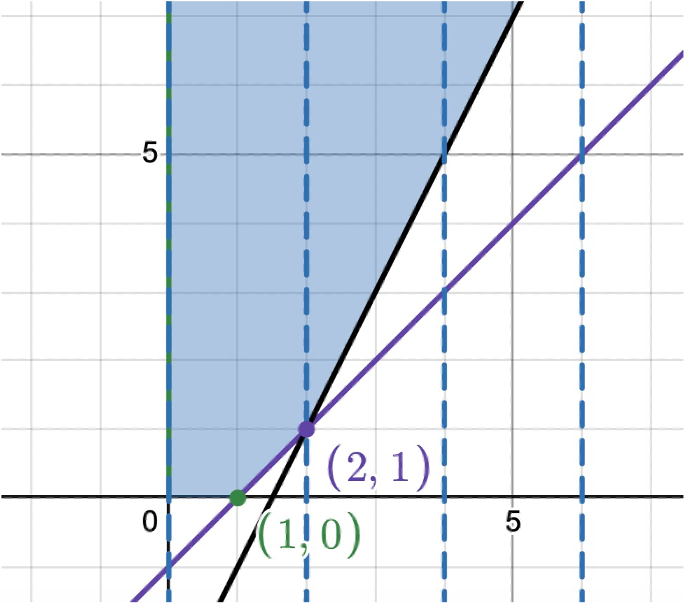
\includegraphics[scale = 0.5]{Figures/unbounded-desmos-simplex}
\end{center}
We convert the inequalities into equalities using slack variables \( s_1 \) and \( s_2 \):

\[
\begin{aligned}
s_1 &= 1 - x_1 + x_2 \\
s_2 &= 3 - 2x_1 + x_2 \\
x_1, x_2, s_1, s_2 &\geq 0
\end{aligned}
\]

\textbf{Initial dictionary (dictionary form):}
\[
\text{Maximize } x_1 \\
\text{subject to} \quad
\begin{cases}
s_1 = 1 - x_1 + x_2 \\
s_2 = 3 - 2x_1 + x_2
\end{cases}
\]

\textbf{Pivot Step 1:} Enter \( x_1 \), leave \( s_2 \) (smallest ratio rule: \( \frac{3}{2} < \frac{1}{1} \)).

Solving \( s_2 = 3 - 2x_1 + x_2 \Rightarrow x_1 = \frac{3 + x_2 - s_2}{2} \), and substitute into the objective and other constraint.

\[
\text{Maximize } 1 + x_2 - s_1 \\
\text{subject to}
\begin{cases}
x_1 = 1 + x_2 - s_1 \\
s_2 = 1 - x_2 + 2s_1
\end{cases}
\]

\textbf{Pivot Step 2:} Enter \( s_1 \), but observe: the variable \( s_1 \) appears in both equations with positive coefficients and no upper bound is imposed. That is, increasing \( s_1 \) increases the objective indefinitely:
\[
\text{Maximize } 1 + x_2 - s_1 \Rightarrow \text{Maximize } 2 + s_1 - s_2
\]

\[
\text{subject to}
\begin{cases}
x_1 = 2 + s_1 - s_2 \\
x_2 = 1 + 2s_1 - s_2
\end{cases}
\]

Since increasing \( s_1 \) increases the objective and does not violate any constraint (no upper bound in any equation), the linear program is \textbf{unbounded}.

\textbf{Conclusion:}  
This linear program is unbounded. Once \( s_1 \) enters the basis, there is no constraint limiting how large it can grow while maintaining feasibility. Therefore, the objective function can increase without bound.
\end{example}


\begin{refsection}
\begin{pioneerspotlight}{George Dantzig}
George Dantzig, known for spearheading linear programming with the simplex algorithm, was born in Portland, Oregon on November 8, 1914 \parencite[pp.~100–106]{gass_2008_memorial}. George received his Bachelor of Arts in Mathematics and Physics from the University of Maryland, College Park. \textcite{gass_2008_memorial} explained that after George married his wife, Anne Shmuner, he completed his Master of Arts in Mathematics at the University of Michigan in 1938. Before graduating with his Master’s degree, he began working at the United States Bureau of Labor Statistics as a junior statistician. \textcite{gass_2008_memorial} described how George took interest in statistics through the work of Jerzy Neyman, which led him to get a Ph.D. in Statistics with Neyman's guidance from the University of California, Berkeley in 1946. Before his dissertation, he began working with the Army Air Force Combat Analysis Branch of Statistical Control at the Pentagon, then transferred to the Department of the Air Force as a mathematical advisor. After his work at the Pentagon, he became a professor in operations research at the University of California, Berkeley, and Stanford. He went on to receive the National Medal of Science in 1975. He was also a member of the National Academy of Engineering and the National Academy of Sciences and the American Association of Arts and Sciences \parencite{ucberkeleyengineering_2018_george}. 
	
While in school at the University of California, Berkeley, George became widely known for solving two of the “unsolved” statistics problems, which he mistakenly thought were homework \parencite{ucberkeleyengineering_2018_george}. In 1947, Dantzig proposed the simplex algorithm, which started the field of linear programming \parencite{cottle_2007_george}. 
Geometrically, the simplex method consists of traveling along the edges of a polyhedron toward its vertices. The optimal solution will be at a vertex if the feasible set is convex. The constraints should be in the following standard form:
\[
A \mathbf{x}_n = \mathbf{b}, \quad x_n = 1, \quad x_j \geq 0 \quad \text{for } j = 1, \ldots, n.
\]

The corresponding vertices of the feasible region are the basic feasible solutions. If a system is nondegenerate, the process of simplex pivoting can occur, where the previous solution is used to pivot towards a better feasible basis. 

After Dantzig’s development of the simplex algorithm, he presented a talk geared toward the application of his linear programming model in the digital world, including games and computers. \textcite{cottle_2007_george} described how his algorithm was implemented in the animal feed industry and computing machines for the Air Force. It was also used to solve Stigler’s “diet problem,” a simple question with modern technology, but a long computation process in 1947. Dantzig’s procedure has been utilized in countless industries, such as communications, railroads, petroleum, airlines, and the economy. His utilization of linear algebra theory and the creation of pivoting will continue to be used when solving complex linear problems.

According to \textcite{cottle_2007_george}, Dantzig also studied network flow problems, which led to the duality theorem in the 1950s. The dual theorem utilizes the costs as integers to create a pair that highlights integer basic solutions, which was used in the application of the “fleet assignment model.” With a great understanding of real-world problems, Dantzig developed the recourse stochastic program, which accounted for uncertain constraints and utilized statistical tests to determine the likelihood of an optimal solution. Dantzig was responsible for the solution to countless military problems through his development of linear programming in the late-1940s. \\
\begin{center}
{\small \textbf{This spotlight was contributed by Irma Adams}}
\end{center}
\printbibliography[heading=subbibliography]
\end{pioneerspotlight}

\end{refsection}
\section{Exercises}
\subsection{Exercises: Converting to Standard Form}

\begin{ex}{}{}
Convert the following linear program to standard form:

\[
\begin{aligned}
    \max \quad & 3x_1 - 5x_2 \\
    \text{subject to} \quad 
    & 2x_1 + x_2 \leq 6, \\
    & -x_1 + 3x_2 \geq 2, \\
    & x_1, x_2 \geq 0.
\end{aligned}
\]
\end{ex}

\begin{ex}{}{}
Convert the following linear program to standard form:

\[
\begin{aligned}
    \min \quad & -x_1 + 2x_2 + x_3 \\
    \text{subject to} \quad 
    & x_1 - x_2 + 2x_3 = 4, \\
    & -2x_1 + x_2 \leq 1, \\
    & x_3 \text{ is unrestricted}, \quad x_1, x_2 \geq 0.
\end{aligned}
\]
\end{ex}

\begin{ex}{}{}
Convert the following linear program to standard form:

\[
\begin{aligned}
    \max \quad & 5x_1 + x_2 - 3x_3 \\
    \text{subject to} \quad 
    & x_1 + 2x_2 - x_3 \geq 7, \\
    & x_2 - 4x_3 = 3, \\
    & x_1 \text{ is unrestricted}, \quad x_2, x_3 \leq 0.
\end{aligned}
\]
\end{ex}


\begin{ex}{}
\label{ex:84}
 Convert the following linear program to standard form:

\[
\begin{aligned}
    \min \quad & 2x_1 + 4x_2 \\
    \text{subject to} \quad 
    & x_1 + x_2 \geq 3, \\
    & 2x_1 - x_2 \leq 5, \\
    & x_1 \text{ is unrestricted}, \quad x_2 \geq 0.
\end{aligned}
\]
\end{ex}



\begin{ex}{}
\label{ex:85}
Convert the following linear program to standard form:

\[
\begin{aligned}
    \min \quad & 5y_1 - 3y_2 + y_3 \\
    \text{subject to} \quad 
    & 2y_1 - y_2 + 3y_3 = 7, \\
    & -y_1 + 4y_2 \leq 5, \\
    & y_3 \text{ is unrestricted}.
\end{aligned}
\]
\end{ex}

\subsubsection*{Selected Solutions}

\begin{solution}(Exercise~\ref{ex:84})

1. Convert the minimization problem to a maximization problem by negating the objective function:
   \[
   \max \quad -2x_1 - 4x_2.
   \]
   
2. Convert the \( \geq \) constraint into an equality by introducing a surplus variable \( s_1 \geq 0 \):
   \[
   x_1 + x_2 - s_1 = 3.
   \]
   
3. Convert the \( \leq \) constraint into an equality by introducing a slack variable \( s_2 \geq 0 \):
   \[
   2x_1 - x_2 + s_2 = 5.
   \]
   
4. Since \( x_1 \) is unrestricted, replace it with \( x_1 = x_1' - x_1'' \), where \( x_1', x_1'' \geq 0 \).

\textbf{Final Standard Form:}
\[
\begin{aligned}
    \max \quad & -2(x_1' - x_1'') - 4x_2 \\
    \text{subject to} \quad 
    & (x_1' - x_1'') + x_2 - s_1 = 3, \\
    & 2(x_1' - x_1'') - x_2 + s_2 = 5, \\
    & x_1', x_1'', x_2, s_1, s_2 \geq 0.
\end{aligned}
\]
\end{solution}
\vspace{1cm}



\begin{solution}(Exercise~\ref{ex:85})

1. Convert the minimization problem to a maximization problem by negating the objective function:
   \[
   \max \quad -5y_1 + 3y_2 - y_3.
   \]

2. Convert the \( \leq \) constraint into an equality by introducing a slack variable \( s_1 \geq 0 \):
   \[
   -y_1 + 4y_2 + s_1 = 5.
   \]

3. Since \( y_3 \) is unrestricted, replace it with \( y_3 = y_3' - y_3'' \), where \( y_3', y_3'' \geq 0 \).

\textbf{Final Standard Form:}
\[
\begin{aligned}
    \max \quad & -5y_1 + 3y_2 - (y_3' - y_3'') \\
    \text{subject to} \quad 
    & 2y_1 - y_2 + 3(y_3' - y_3'') = 7, \\
    & -y_1 + 4y_2 + s_1 = 5, \\
    & y_1, y_2, y_3', y_3'', s_1 \geq 0.
\end{aligned}
\]
\end{solution}





\subsection{Simplex Method}
\begin{ex}[Pivoting in a different direction]{}
\label{ex:alternative-pivot}
We consider the example from Section~\ref{sec:pivoting}.  In that example, we pivoted first on the $y$ vaiable.  This choice of pivot called the \emph{steepest ascent} rule since we chose the variable in the objective with the largest coefficient.  
However, we can consider pivoting on any variable with a positive coefficient in the objective.  We will now pivot first on the $x$ variable.  

\textbf{Starting Point}
\[
\begin{aligned}
\text{Maximize}\quad &  2x + 3y \\
\text{subject to}\quad & s_1 = 9 - x - y, \\
                        & s_2 = 16 - 2x - y, \\
                        & s_3 = 14 - x - 2y, \\
                        & x, y, s_1, s_2, s_3 \ge 0.
\end{aligned}
\]

\begin{enumerate}
    \item Let \(x\) increase first.
    \item Determine which variable leaves the basis using the ratio test.
    \item Pivot by rewriting the equation of the leaving variable in terms of \(x\) and substitute it into the other equations and the objective.
    \item Write down the new dictionary.
    \item Decide whether the resulting dictionary is optimal. If not, repeat the process.
\end{enumerate}
\end{ex}

\begin{ex}{}
Solve the following linear programming problem using the simplex method:
\[
\begin{aligned}
\text{Maximize:}\quad & z = 5x_{1} + 3x_{2}\\
\text{subject to:}\quad & x_{1} + x_{2} \le 12,\\
& 2x_{1} + x_{2} \le 16,\\
& x_{1},\, x_{2} \ge 0.
\end{aligned}
\]
\end{ex}

\begin{ex}{}
Solve the following linear programming problem using the simplex method:
\[
\begin{aligned}
\text{Maximize:}\quad & z = 5x_{1} + 8x_{2}\\
\text{subject to:}\quad & x_{1} + 2x_{2} \le 30,\\
& 3x_{1} + x_{2} \le 30,\\
& x_{1},\, x_{2} \ge 0.
\end{aligned}
\]
\end{ex}

\begin{ex}{}
Solve the following linear programming problem using the simplex method:
\[
\begin{aligned}
\text{Maximize:}\quad & z = 2x_{1} + 3x_{2} + x_{3} \\
\text{subject to:}\quad & 4x_{1} + 2x_{2} + 5x_{3} \le 32,\\
& 2x_{1} + 4x_{2} + 3x_{3} \le 28,\\
& x_{1},\, x_{2},\, x_{3} \ge 0.
\end{aligned}
\]
\end{ex}

\begin{ex}{}
Solve the following linear programming problem using the simplex method:
\[
\begin{aligned}
\text{Maximize:}\quad & z = 6x_{1} + 8x_{2} + 5x_{3},\\
\text{subject to:}\quad & 4x_{1} + x_{2} + x_{3} \le 1800,\\
& 2x_{1} + 2x_{2} + x_{3} \le 2000,\\
& 4x_{1} + 2x_{2} + x_{3} \le 3200,\\
& x_{1},\, x_{2},\, x_{3} \ge 0.
\end{aligned}
\]
\end{ex}

\begin{ex}{}
Solve the following linear programming problem using the simplex method:
\[
\begin{aligned}
\text{Minimize:}\quad & z = 4x_{1} + 6x_{2} + 7x_{3}, \\
\text{subject to:}\quad & x_{1} + x_{2} + 2x_{3} \ge 20,\\
& x_{1} + 2x_{2} + x_{3} \ge 30,\\
& x_{1},\, x_{2},\, x_{3} \ge 0.
\end{aligned}
\]
\end{ex}

\begin{ex}{}
Solve the following linear programming problem using the simplex method:
\[
\begin{aligned}
\text{Minimize:}\quad & z = 40x_{1} + 48x_{2} + 30x_{3}, \\
\text{subject to:}\quad & 2x_{1} + 2x_{2} + x_{3} \ge 25,\\
& x_{1} + 3x_{2} + 2x_{3} \ge 30,\\
& x_{1},\, x_{2},\, x_{3} \ge 0.
\end{aligned}
\]
\end{ex}

\begin{ex}
{Conditions in the dictionary.} The following is a dictionary of a maximization problem. State conditions (i.e., the range of values) on $a_{1}, a_{2}, b, c_{1}, c_{5}, c_{6}$ that are required to make the following true.  Note: This does not require any simplex pivots.
\begin{center}
\begin{align*}
\max \quad &0 + c_1 x_1 + c_5 x_5 + c_6 x_6 \\
x_2 &= 1 + x_1 - a_1 x_5 \\
x_4 &= 2 + x_1 + 2x_5 - x_6 \\
x_3 &= b - a_2 x_1 - x_5 - x_6
\end{align*}
\end{center}

\begin{enumerate}
\item  The current solution is feasible and optimal.
\item The current basic solution is not feasible.
\item  The current basic solution is degenerate.
\item  The current basic solution is feasible, and the LP is unbounded.
\end{enumerate}

\end{ex}

\begin{ex}

Consider the following linear programming feasible region in 2 variables that is depicted in the plot below.   
%$$
%\begin{array}{rrrrrrrrr}
% \text { maximize } &2 x_{1}&+&x_{2} \\
% \text { subject to } & -x_{1}&+&x_{2} &\leq &2 \\
%%&-x_{1}&+&x_{2}&  \leq &2 \\
%&&&x_{2}  &\leq &4 \\ 
%%&x_{1}&+&x_{2}  &\leq& 8 \\
%& x_{1}&+&x_{2} &\leq &8 \\
%%&2 x_{1}&-&x_{2} & \leq &10 \\
%& 2 x_{1}&-&x_{2} &\leq &10 \\
%& &x_{1},& x_{2} &\geq &0 .
%\end{array}
%$$

Here is a graph of the feasible region:
\begin{center}
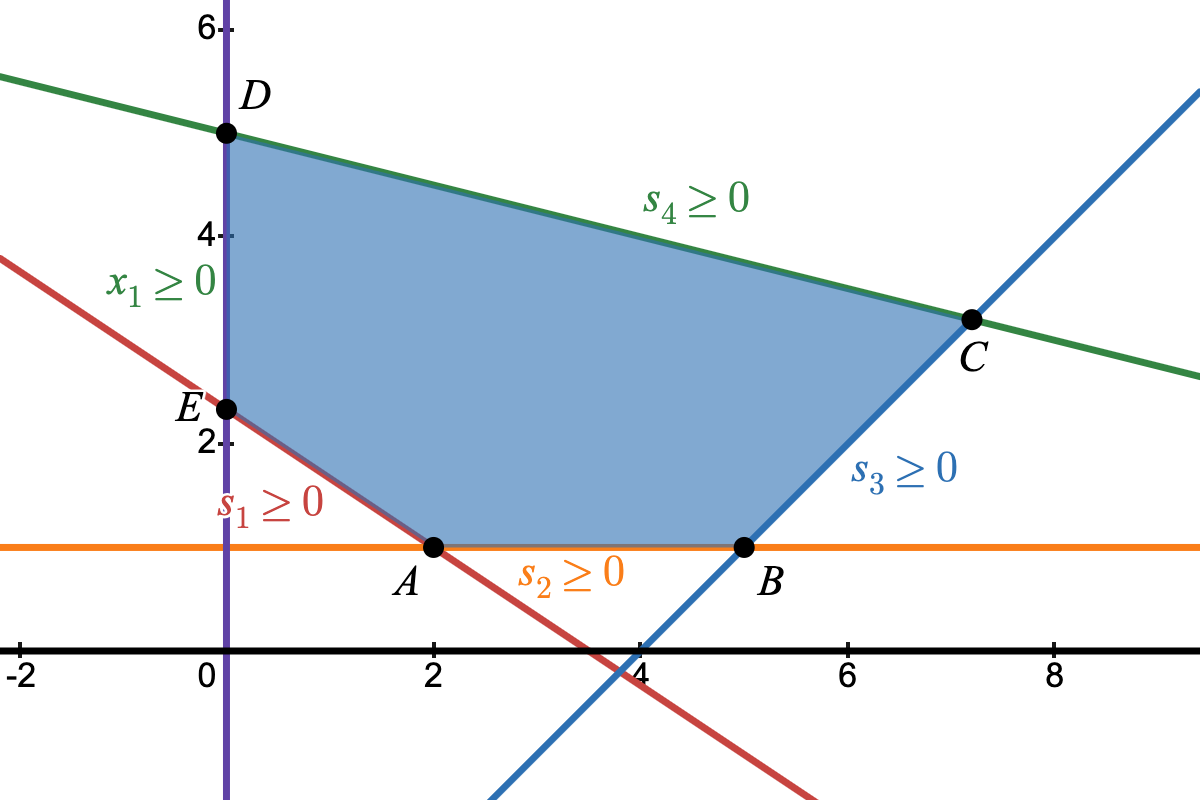
\includegraphics[width=0.6\textwidth]{Figures/desmos-graph-slacks}
\end{center}

The variables in the augmented linear program are $\{x_1, x_2, s_1, s_2, s_3, s_4\}$.
In the context of  the simplex method, answer the following questions:

(a)   At the basic feasible solution $D$, which variables are non-basic and which variables are basic?
$$
B = \big\{ \hspace{5cm} \big\}, \hspace{3cm}  N = \big\{ \hspace{3cm} \big\}. 
$$

(b) If we pivot from the basic feasible solution at $D$ to the basic feasible solution at $C$, 
\begin{itemize}
\item Which variable enters the basis?\\
\item Which variable leaves the basis?
\end{itemize}

\end{ex}

\subsection*{Solutions to selected exercises}

\begin{solution}[Solution for Exercise~\ref{ex:alternative-pivot}]
We will have to do 3 pivots!

We begin with the original linear program:
\[
\begin{aligned}
\text{Maximize}\quad & 2x + 3y \\
\text{subject to}\quad & s_1 = 9 - x - y, \\
                        & s_2 = 16 - 2x - y, \\
                        & s_3 = 14 - x - 2y, \\
                        & x, y, s_1, s_2, s_3 \ge 0.
\end{aligned}
\]

\textbf{First Pivot: \(x\) Enters the Basis}

Let \(x\) increase first. Applying the ratio test shows that a certain slack variable (here, for example, the calculations lead us to pivot so that the new dictionary is obtained) leaves the basis. After performing the necessary algebraic manipulations (i.e., rewriting the leaving variable’s equation in terms of \(x\) and substituting into the other equations), we obtain:
\[
\begin{aligned}
\text{Maximize}\quad & 16 + 2y - s_2 \\
\text{subject to}\quad & s_1 = 1 - 0.50y + 0.50s_2, \\
                        & x = 8 - 0.50y - 0.50s_2, \\
                        & s_3 = 6 - 1.50y + 0.50s_2, \\
                        & x, y, s_1, s_2, s_3 \ge 0.
\end{aligned}
\]

\textbf{Second Pivot: \(y\) Enters the Basis}

Next, we pivot again. In this pivot, the calculations lead us to select \(y\) (or, equivalently, pivot so that the basic variable changes as indicated by the ratio test). After rewriting the appropriate equation in terms of the entering variable and substituting into the remaining equations and the objective function, the dictionary becomes:
\[
\begin{aligned}
\text{Maximize}\quad & 20 - 4s_1 + s_2 \\
\text{subject to}\quad & y = 2 - 2s_1 + s_2, \\
                        & x = 7 + s_1 - s_2, \\
                        & s_3 = 3 + 3s_1 - s_2, \\
                        & x, y, s_1, s_2, s_3 \ge 0.
\end{aligned}
\]
\textbf{Third Pivot: \(s_2\) Enters the Basis}

The new dictionary is
\[
\begin{aligned}
\text{Maximize}\quad & 23 - s_1 - s_3 \\
\text{subject to}\quad & x = 4 - 2s_1 + s_3, \\
                        & s_2 = 3 + 3s_1 - s_3, \\
                        & y = 5 + s_1 - s_3, \\
                        & x, y, s_1, s_2, s_3 \ge 0.
\end{aligned}
\]

This is optimal!

\end{solution}





